\section{Architettura}

%%%%%%%%%%%%%%%%%%%%%%%%%%%%%%%%%%%%%%%%%%%%%%%%%%%%%%%%%%%%%%%%%%%%%%%%%%%%%%%%%%
\subsection{Introduzione all’architettura}
    \subsubsection{Scopo e obbiettivi}
    La presente sezione ha lo scopo di fornire una visione d’insieme dell’architettura del sistema, evidenziandone i principi guida e le scelte progettuali che ne hanno determinato la struttura. In particolare, si intende:
    \begin{itemize}
        \item Definire il contesto in cui opera il sistema, evidenziando i requisiti funzionali e non funzionali che hanno condotto alla scelta di una specifica architettura.
        \item Orientare i lettori (sviluppatori, progettisti e stakeholder) verso una comprensione chiara delle componenti principali e delle interazioni che caratterizzano il sistema.
        \item Porre le basi per la discussione delle scelte di design, evidenziando come queste possano rispondere alle esigenze di scalabilità, sicurezza, manutenibilità e performance.
        \item Descrivere le motivazioni alla base delle scelte tecnologiche e dei modelli architetturali adottati.
    \end{itemize}



%%%%%%%%%%%%%%%%%%%%%%%%%%%%%%%%%%%%%%%%%%%%%%%%%%%%%%%%%%%%%%%%%%%%%%%%%%%%%%%%%%

\subsection{Architettura del sistema}
La progettazione dell’architettura del sistema ha richiesto un’approfondita analisi delle due principali opzioni architetturali disponibili: \textbf{monolitica} e \textbf{a microservizi}. La scelta dell’architettura è stata guidata da una serie di fattori, tra cui la natura dell’applicazione, il volume di traffico previsto, i costi di sviluppo e manutenzione e la necessità di scalabilità. In questa sezione verranno analizzati nel dettaglio i pro e i contro di entrambe le soluzioni, per poi motivare la decisione finale.
\subsubsection{Architettura monolitica}
Un’architettura monolitica si basa su un’unica codebase che incorpora tutti i componenti dell’applicazione, tra cui l’interfaccia utente, la logica di business e il livello di accesso ai dati. Questo approccio, tradizionalmente adottato nello sviluppo software, è particolarmente indicato per applicazioni di piccola e media complessità, in cui i costi di separazione dei componenti in unità indipendenti non sono giustificati.
\paragraph{Vantaggi}  
\begin{itemize}
    \item \textbf{Semplicità di sviluppo e gestione}: Un’unica codebase permette di mantenere una visione centralizzata del sistema, semplificando lo sviluppo, il testing e il debugging.
    \item \textbf{Minori costi di infrastruttura}: Non è necessario investire in strumenti di orchestrazione, load balancing o gestione della comunicazione tra microservizi.
    \item \textbf{Deployment più semplice}: L’intero sistema viene distribuito come un’unica unità, evitando problemi di coordinamento.
    \item \textbf{Prestazioni migliori per bassi volumi di traffico}: L’assenza di chiamate di rete tra microservizi riduce la latenza.
\end{itemize}
\paragraph{Svantaggi}  
\begin{itemize}
    \item \textbf{Scalabilità limitata}: Non è possibile scalare singole componenti separatamente.
    \item \textbf{Maggiore impatto degli errori}: Un bug in una parte dell’applicazione può compromettere l’intero sistema.
    \item \textbf{Difficoltà nell’adozione di nuove tecnologie}: L’aggiornamento di singole parti è complesso poiché l’intero stack è integrato.
\end{itemize}

\subsubsection{Architettura a microservizi}
L’architettura a microservizi suddivide il sistema in componenti indipendenti, ognuno responsabile di una funzionalità specifica. Ogni microservizio comunica con gli altri attraverso API, permettendo un alto grado di indipendenza e flessibilità nello sviluppo.
\paragraph{Vantaggi}  
\begin{itemize}
    \item \textbf{Scalabilità orizzontale}: Ogni microservizio può essere scalato indipendentemente.
    \item \textbf{Flessibilità nello sviluppo}: Permette l’adozione di tecnologie diverse per ciascun servizio.
    \item \textbf{Maggiore resilienza}: Un errore in un microservizio non compromette l’intero sistema.
    \item \textbf{Facilità di manutenzione}: È possibile distribuire aggiornamenti senza dover ripubblicare l’intera applicazione.
\end{itemize}
\paragraph{Svantaggi}  
\begin{itemize}
    \item \textbf{Maggiore complessità gestionale}: L’orchestrazione dei microservizi richiede strumenti avanzati.
    \item \textbf{Comunicazione tra servizi}: Introduce latenza e potenziali colli di bottiglia.
    \item \textbf{Deployment più complesso}: Coordinare il rilascio di più servizi è più oneroso.
    \item \textbf{Costi di sviluppo più elevati}: La frammentazione del sistema richiede maggiore sforzo di progettazione e testing.
\end{itemize}

\subsubsection{Scelta del monolite esagonale}
Dopo un’analisi approfondita, il team di sviluppo ha deciso di adottare un’\textbf{architettura monolitica esagonale}. Questa scelta è stata motivata dai seguenti fattori:
\begin{enumerate}
    \item \textbf{Basso carico di utenti}: L’applicazione è destinata a un contesto B2B con un numero limitato di utenti concorrenti.
    \item \textbf{Semplicità di gestione}: La manutenzione di un monolite è più diretta rispetto a un sistema distribuito.
    \item \textbf{Riduzione dei costi operativi}: L’assenza di strumenti di orchestrazione riduce significativamente i costi di infrastruttura.
    \item \textbf{Velocità di sviluppo}: Un’unica codebase consente iterazioni rapide senza dipendenze tra servizi separati.
    \item \textbf{Evoluzione graduale verso microservizi}: Adottando un’architettura \textbf{esagonale}, il sistema può essere trasformato gradualmente in microservizi senza riscrivere tutto.
\end{enumerate}

\subsection{Architettura esagonale}
L’\textbf{architettura esagonale}, nota anche come \textit{Ports and Adapters}, è un pattern architetturale l'obiettivo di rendere il software più flessibile, testabile e indipendente dalle tecnologie esterne. Questo approccio enfatizza la separazione tra la logica di business e le interfacce di comunicazione con il mondo esterno.

\subsubsection{Principi fondamentali}
L'architettura esagonale si basa su tre concetti chiave:
\begin{itemize}
    \item \textbf{Isolamento della logica di business}: Il core dell'applicazione è indipendente dai dettagli implementativi esterni.
    \item \textbf{Utilizzo di porte e adattatori}: Le \textit{porte} definiscono le interfacce per la comunicazione tra il core e il mondo esterno, mentre gli \textit{adattatori} implementano queste interfacce per specifiche tecnologie.
    \item \textbf{Sostituibilità delle dipendenze}: È possibile cambiare database, framework web o altre dipendenze senza impattare il core.
\end{itemize}

\subsubsection{Struttura dell’architettura esagonale}
L’architettura esagonale può essere rappresentata con tre livelli principali:
\begin{enumerate}
    \item \textbf{Core (Dominio e Logica di Business)}: Contiene le regole fondamentali dell’applicazione.
    \item \textbf{Porte (Ports)}: Interfacce che definiscono i punti di ingresso e uscita del sistema.
    \item \textbf{Adattatori (Adapters)}: Implementazioni concrete delle porte per database, servizi esterni e UI.
\end{enumerate}
\begin{figure}[H]
    \centering
    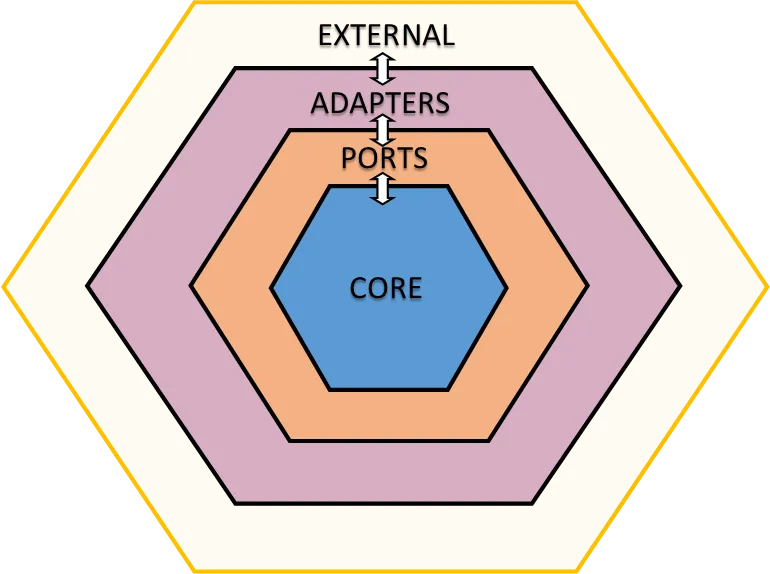
\includegraphics[width=0.7\textwidth]{./img/hexagonal_architecture.png}
    \caption{Schema dell'architettura esagonale}
    \label{fig:hex_arch}
\end{figure}

\subsubsection{Vantaggi dell’architettura esagonale}
Adottare un'architettura esagonale comporta diversi benefici:
\begin{itemize}
    \item \textbf{Maggiore manutenibilità}: Il codice è modulare e separato.
    \item \textbf{Facilità di test}: Il core dell’applicazione può essere testato isolatamente.
    \item \textbf{Indipendenza dalle tecnologie}: Cambiare framework o database ha un impatto minimo.
    \item \textbf{Flessibilità evolutiva}: Permette di trasformare gradualmente il monolite in microservizi.
\end{itemize}

\subsubsection{Conclusione}
L’architettura esagonale garantisce modularità e sostenibilità del sistema nel lungo termine, permettendo di scalare senza impattare la stabilità complessiva dell’applicazione.

\subsection{Architettura Esagonale in dettaglio}
\begin{figure}[H]
    \centering
    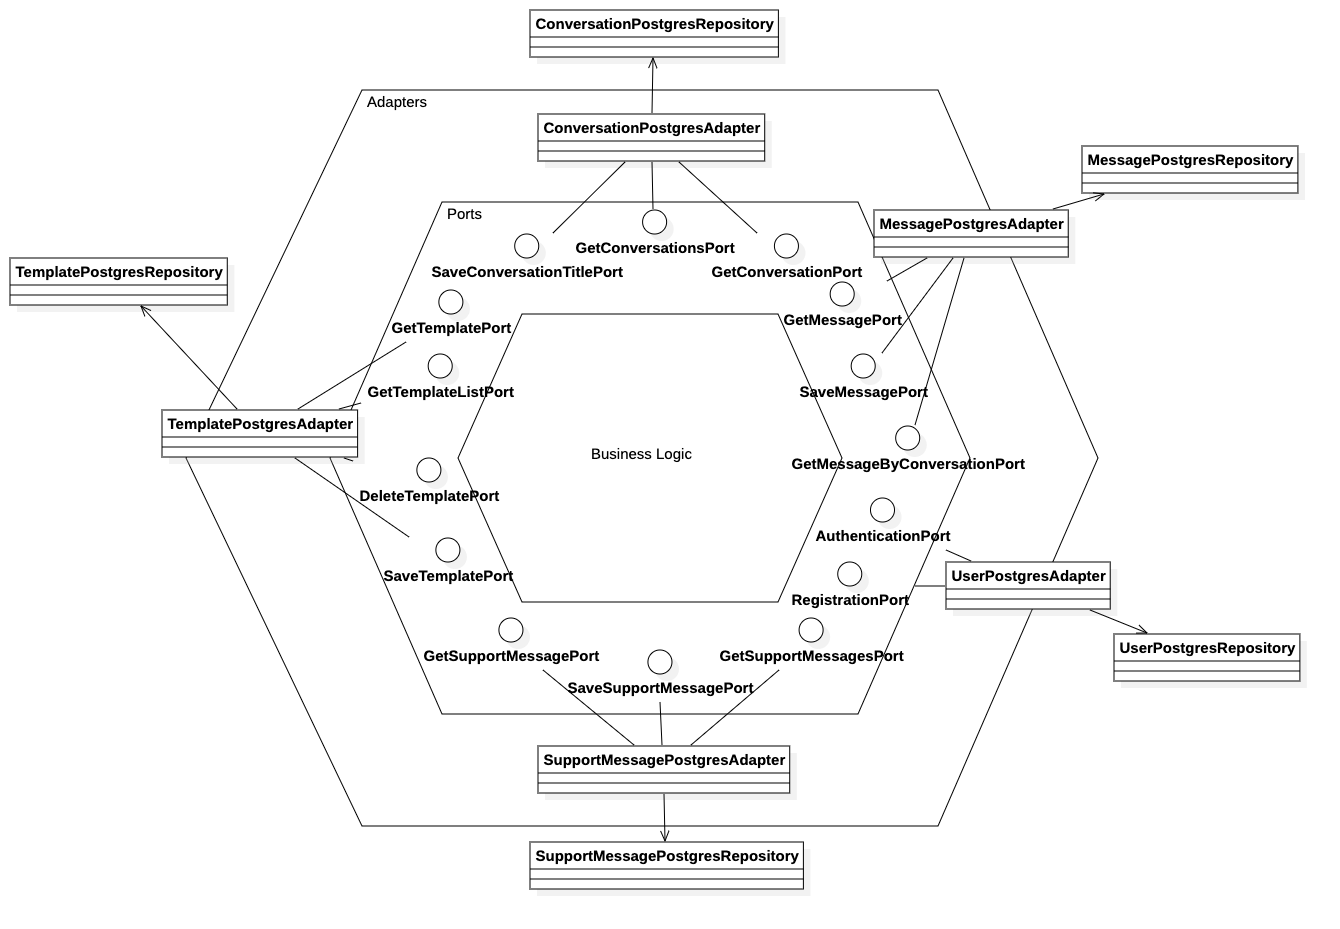
\includegraphics[width=\linewidth, height=0.8\textheight, keepaspectratio]{./img/ArchitetturaEsagonaleStarUML.png}
    \caption{Diagramma delle classi - Architettura Esagonale}
    \label{fig:architettura_esagonale}
\end{figure}
Di seguito viene descritta in dettaglio la funzione e l'interazione delle classi della gerarchia proposta, evidenziando il tipo di dato che ciascuna gestisce (entity, model o DTO).

\paragraph{Repository (usa Entity)} 
\mbox{}\\
\textbf{Funzione:} Il repository è responsabile della persistenza e del recupero dei dati dal mezzo di archiviazione (ad esempio, un database relazionale o NoSQL). 
\mbox{}\\
\textbf{Dettagli:}
\begin{itemize}
  \item \textbf{Entity:} Le entity rappresentano il modello del dominio, contenente le informazioni e le regole di business fondamentali.
  \item \textbf{Operazioni tipiche:} CRUD (creazione, lettura, aggiornamento, cancellazione).
  \item \textbf{Astrazione:} Il repository isola il dominio dai dettagli tecnici della persistenza, permettendo al core di rimanere indipendente da framework o tecnologie specifiche.
\end{itemize}

\paragraph{Adapter (usa Model)}
\mbox{}\\
\textbf{Funzione:} L’adapter funge da mediatore tra il core dell’applicazione e i sistemi esterni o infrastrutture (ad esempio, servizi di terze parti, API, file system). \\
\mbox{}\\
\textbf{Dettagli:}
\begin{itemize}
  \item \textbf{Conversione dei dati:} Trasforma i dati dal formato utilizzato internamente (model) a quello richiesto dal sistema esterno e viceversa.
  \item \textbf{Isolamento delle dipendenze:} Nasconde la complessità delle tecnologie esterne al dominio, conformandosi alle interfacce (port) definite dal core.
\end{itemize}

\paragraph{Port (usa Model)}
\mbox{}\\
\textbf{Funzione:} I port rappresentano le interfacce o contratti che definiscono il modo in cui il core comunica con il mondo esterno. \\
\mbox{}\\
\textbf{Dettagli:}
\begin{itemize}
  \item \textbf{Definizione del contratto:} Stabiliscono quali operazioni sono disponibili e come devono essere invocate, senza specificare l’implementazione.
  \item \textbf{Indipendenza dal framework:} Consentono al dominio di essere testato e sviluppato senza dipendenze dirette da componenti esterni.
\end{itemize}

\paragraph{Service (usa Model)}
\mbox{}\\
\textbf{Funzione:} I service aggregano e orchestrano la logica di business complessa, spesso condivisa tra più casi d’uso. \\
\mbox{}\\
\textbf{Dettagli:}
\begin{itemize}
  \item \textbf{Coordinamento delle operazioni:} Chiamano i repository per accedere ai dati, invocano i port per interagire con sistemi esterni e applicano le regole di business.
  \item \textbf{Modularità:} Incapsulano comportamenti riutilizzabili, mantenendo il core dell’applicazione pulito e focalizzato sulle regole di business.
\end{itemize}

\paragraph{Usecase (usa Model)}
\mbox{}\\
\textbf{Funzione:} Gli usecase rappresentano le singole operazioni o workflow che l’applicazione offre; sono casi d’uso specifici del dominio. \\
\mbox{}\\
\textbf{Dettagli:}
\begin{itemize}
  \item \textbf{Incapsulamento del flusso di lavoro:} Ogni usecase definisce un’intera operazione (ad es. "crea ordine", "effettua pagamento"), coordinando il service e altre componenti necessarie per completarla.
  \item \textbf{Gestione del modello:} Utilizzano il model per rappresentare i dati che vengono manipolati durante il caso d’uso, garantendo la coerenza con le regole di business.
\end{itemize}

\paragraph{Controller (usa DTO)}
\mbox{}\\
\textbf{Funzione:} Il controller è il punto di ingresso per le richieste esterne (tipicamente interfacce web, API REST, interfacce utente) e si occupa di tradurle nel linguaggio comprensibile dal dominio. \\
\mbox{}\\
\textbf{Dettagli:}
\begin{itemize}
  \item \textbf{Utilizzo dei DTO:} I Data Transfer Object (DTO) sono strutture dati leggere che trasportano le informazioni tra il client e il server, evitando di esporre direttamente il modello di dominio o le entity.
  \item \textbf{Validazione e mapping:} Il controller riceve i dati in formato DTO, li valida e li converte in input per i usecase; allo stesso modo, trasforma i risultati (model) in DTO da restituire all’utente.
\end{itemize}

\paragraph{Flusso Complessivo dei Dati}
\begin{enumerate}
  \item \textbf{Ingresso:} Il controller riceve una richiesta (es. HTTP) con i dati in formato DTO.
  \item \textbf{Esecuzione del Usecase:} Il controller passa questi dati a un usecase, che rappresenta un’operazione specifica del dominio.
  \item \textbf{Business Logic:} Il usecase, eventualmente tramite un service, applica la logica di business usando il model e interagendo con i port.
  \item \textbf{Interazione Esterna:} Se necessario, un adapter viene utilizzato per comunicare con sistemi esterni (ad es. per salvare dati), passando attraverso il port che definisce il contratto.
  \item \textbf{Persistenza:} Il repository si occupa della persistenza, lavorando direttamente con le entity che rappresentano i dati fondamentali.
  \item \textbf{Risposta:} Una volta completata l’operazione, il risultato viene ritrasformato (tramite mapping) in un DTO e restituito al client attraverso il controller.
\end{enumerate}

\paragraph{Vantaggi di questa Architettura}
\begin{itemize}
  \item \textbf{Isolamento del dominio:} Il core dell’applicazione è isolato da dettagli tecnici e variazioni infrastrutturali, facilitando test, manutenzione e scalabilità.
  \item \textbf{Flessibilità:} I port e gli adapter permettono di sostituire facilmente componenti esterni (ad es. cambiare il database o il sistema di invio email) senza impattare la logica di business.
  \item \textbf{Chiarezza e Separazione dei Compiti:} La divisione in repository, adapter, port, service, usecase e controller aiuta a mantenere un’architettura modulare, in cui ogni componente ha un compito ben definito.
\end{itemize}

%%%%%%%%%%%%%%%%%%%%%%%%%%%%%%%%%%%%%%%%%%%%%%%%%%%%%%%%%%%%%%%%%%%%%%%%%%%%%%%%%%

\subsection{Moduli}

    \subsubsection{Chat Controller}

    \begin{figure}[H]
        \centering
        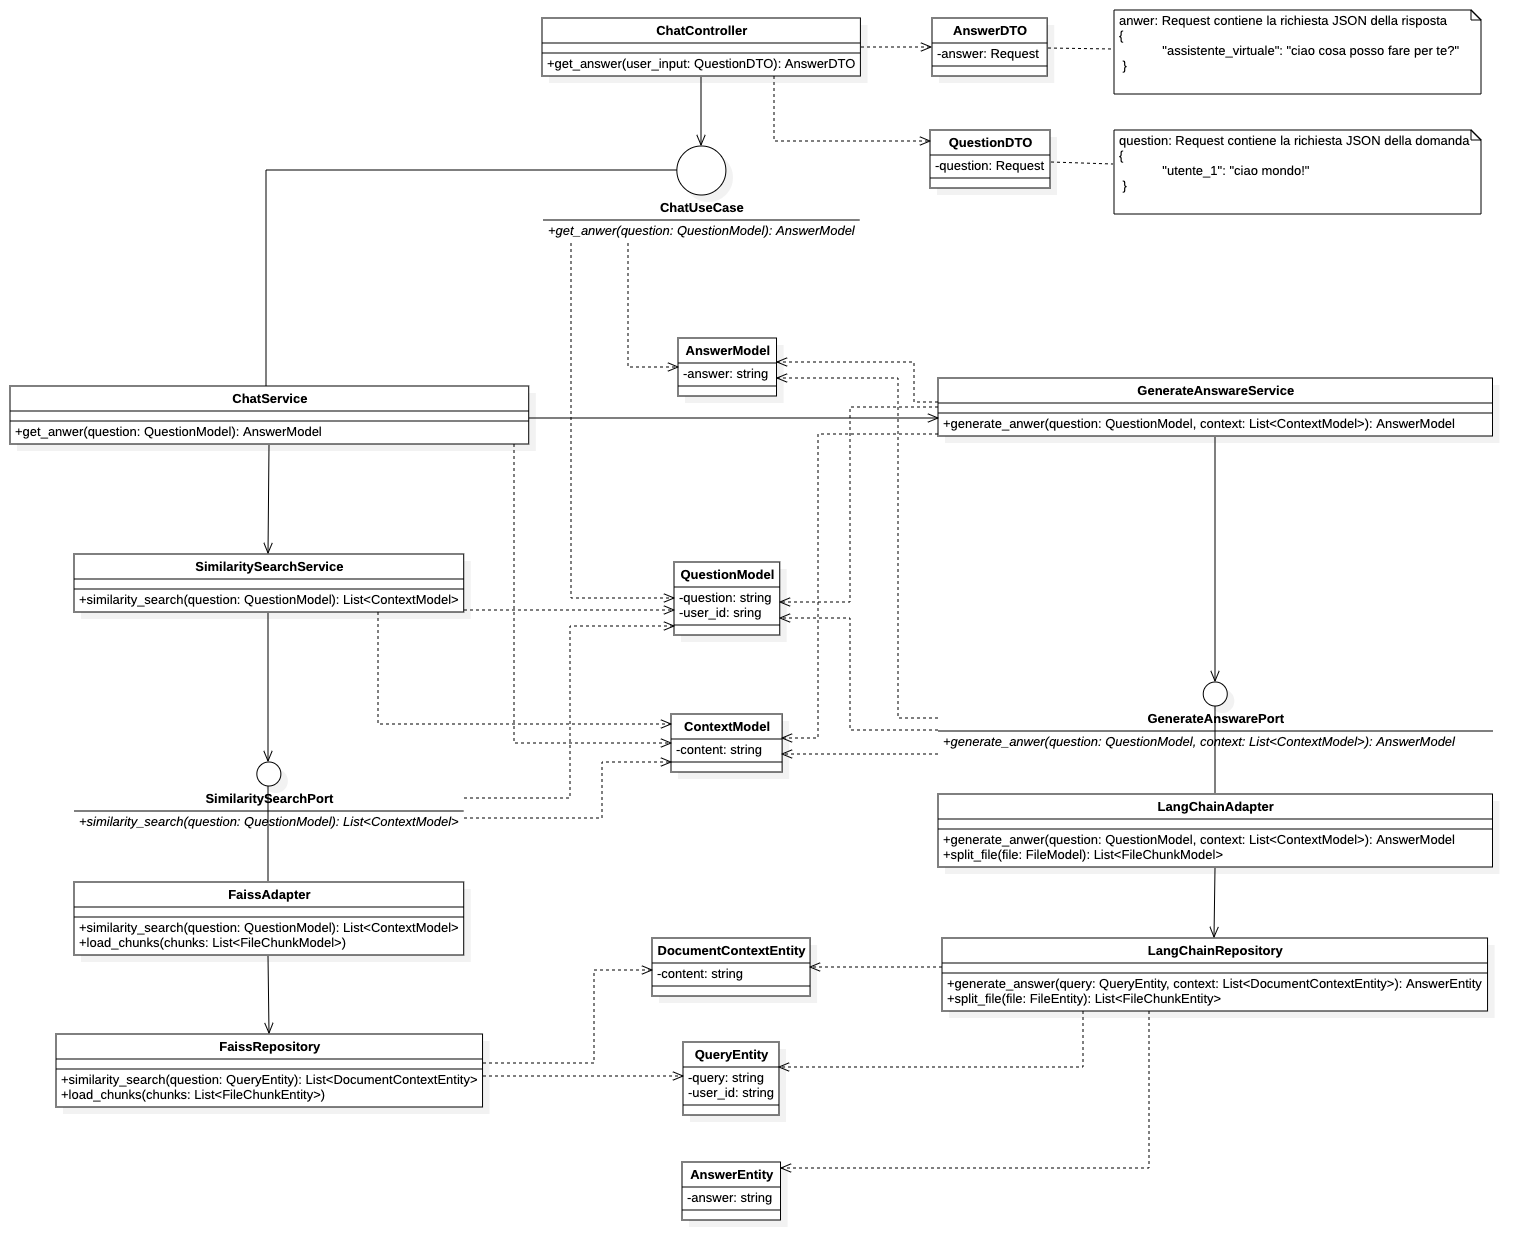
\includegraphics[width=\linewidth, height=0.8\textheight, keepaspectratio]{./img/ChatController.png}
        \caption{Diagramma delle classi - Chat Controller}
        \label{fig:chat_controller}
    \end{figure}

    \paragraph{1. Data Transfer Objects (DTO)}
    \begin{itemize}
        \item \textbf{AnswerDTO \& QuestionDTO:}
        \begin{itemize}
            \item Questi oggetti sono usati per trasferire i dati tra le varie componenti (ad esempio, tra il controller e il caso d’uso).
            \item AnswerDTO incapsula la risposta generata.
            \item QuestionDTO contiene informazioni relative all’utente (identificato da un intero) e alla domanda posta.
        \end{itemize}
    \end{itemize}

    \paragraph{2. Modelli ed Entità}
    \begin{itemize}
        \item \textbf{Modelli (Models):}
        \begin{itemize}
            \item Rappresentano le strutture dati a livello di dominio, per esempio:
            \begin{itemize}
                \item \textit{QuestionModel}: Tiene traccia dell’ID utente e del testo della domanda.
                \item \textit{AnswerModel}: Incapsula la risposta generata.
                \item \textit{ContextModel}: Utilizzato per rappresentare il contesto (ad esempio, contenuti estratti da documenti) che verrà usato per generare una risposta.
            \end{itemize}
        \end{itemize}
        \item \textbf{Entità:}
        \begin{itemize}
            \item Gli oggetti di tipo entità, come DocumentContextEntity, QueryEntity e AnswerEntity, rappresentano versioni “di basso livello” degli stessi concetti, ma con logiche e metodi per accedere ai dati (ad esempio, \texttt{get\_content()} o \texttt{get\_query()}).
            \item Queste entità sono utili per trasformare i dati dai modelli alle strutture usate nelle operazioni di business.
        \end{itemize}
    \end{itemize}

    \paragraph{3. Repositories e Interazione con il Vector Store}
    \begin{itemize}
        \item \textbf{FaissRepository:}
        \begin{itemize}
            \item Questo componente interagisce direttamente con un vector store basato su FAISS.
            \item \texttt{similarity\_search(query)}: Riceve una QueryEntity, esegue una ricerca di similarità sul vector store (limitata ad un certo numero di risultati, ad esempio 4) e trasforma i documenti trovati in oggetti DocumentContextEntity.
            \item \texttt{load\_chunks(chunks)}: Consente di caricare “chunk” di testo (rappresentati come FileChunkEntity) nel vector store. Per ciascun chunk viene creato un oggetto Document con metadati, successivamente il vector store viene salvato in maniera persistente.
        \end{itemize}
    \end{itemize}

    \paragraph{4. Integrazione con LangChain}
    \begin{itemize}
        \item \textbf{LangChainRepository:}
        \begin{itemize}
            \item Utilizza le funzionalità di LangChain per la generazione di risposte e per la suddivisione dei file.
            \item \texttt{generate\_answer(query, contexts, prompt\_template)}:
            \begin{enumerate}
                \item Prepara una lista di documenti (tramite Document di LangChain) a partire dai contesti ricevuti.
                \item Recupera la “memoria” utente per mantenere la storia delle conversazioni, la quali vengono trimmate se troppo lunghe per non superare un limite di token.
                \item Costruisce dinamicamente un prompt (usando ChatPromptTemplate) che include istruzioni di sistema, la storia della conversazione, la domanda attuale e il contesto.
                \item Invoca una catena (chain) per ottenere la risposta dall’LLM.
                \item Salva l’interazione nella memoria utente e restituisce la risposta incapsulata in un AnswerEntity.
            \end{enumerate}
            \item \texttt{split\_file(file)}: Suddivide il contenuto di un file in “chunk” di dimensioni definite (ad es. 2500 caratteri) utilizzando lo RecursiveCharacterTextSplitter. Se il contenuto è in bytes, viene decodificato in stringa. Il risultato è una lista di oggetti FileChunkEntity.
        \end{itemize}
    \end{itemize}

    \paragraph{5. Adattatori (Adapters)}
    \begin{itemize}
        \item \textbf{FaissAdapter:}
        \begin{itemize}
            \item Implementa l’interfaccia SimilaritySearchPort e AddChunksPort.
            \item Il metodo \texttt{similarity\_search()} trasforma un QuestionModel in una QueryEntity.
            \item Converte i risultati del repository in istanze di ContextModel.
        \end{itemize}
        \item \textbf{LangChainAdapter:}
        \begin{itemize}
            \item Implementa le interfacce GenerateAnswerPort e SplitFilePort.
            \item \texttt{generate\_answer()} converte il QuestionModel e la lista di ContextModel in entità adatte alla generazione della risposta.
            \item \texttt{split\_file()} trasforma un FileModel in un FileEntity e poi converte i chunk ottenuti in oggetti FileChunkModel.
        \end{itemize}
    \end{itemize}

    \paragraph{6. Interfacce (Ports)}
    \begin{itemize}
        \item Definiscono i contratti per le funzionalità principali:
        \begin{itemize}
            \item \textbf{SimilaritySearchPort:} Definisce il metodo per eseguire la ricerca di similarità dati un QuestionModel.
            \item \textbf{GenerateAnswerPort:} Definisce il metodo per generare una risposta basata su domanda, contesto e prompt template.
        \end{itemize}
    \end{itemize}

    \paragraph{7. Servizi}
    \begin{itemize}
        \item \textbf{SimilaritySearchService:} Gestisce la ricerca di similarità per un QuestionModel.
        \item \textbf{GenerateAnswerService:} Invoca la generazione della risposta e gestisce la propagazione degli errori.
    \end{itemize}

    \paragraph{8. Use Case e ChatService}
    \begin{itemize}
        \item \textbf{ChatUseCase (interfaccia astratta) e ChatService (implementazione):}
        \begin{itemize}
            \item \texttt{get\_answer(question\_model)} coordina il processo di recupero del contesto e generazione della risposta.
        \end{itemize}
    \end{itemize}

    \paragraph{9. Controller}
    \begin{itemize}
        \item \textbf{ChatController:}
        \begin{itemize}
            \item Funziona da interfaccia verso l’esterno (ad esempio, per una API REST).
            \item \texttt{get\_answer(user\_input)}:
            \begin{enumerate}
                \item Converte il QuestionDTO in un QuestionModel.
                \item Chiama il caso d’uso ChatUseCase per ottenere la risposta.
                \item Converte il risultato (AnswerModel) in un AnswerDTO da restituire al chiamante.
            \end{enumerate}
        \end{itemize}
    \end{itemize}

    \subsubsection{Add File Controller}

    \begin{figure}[H]
        \centering
        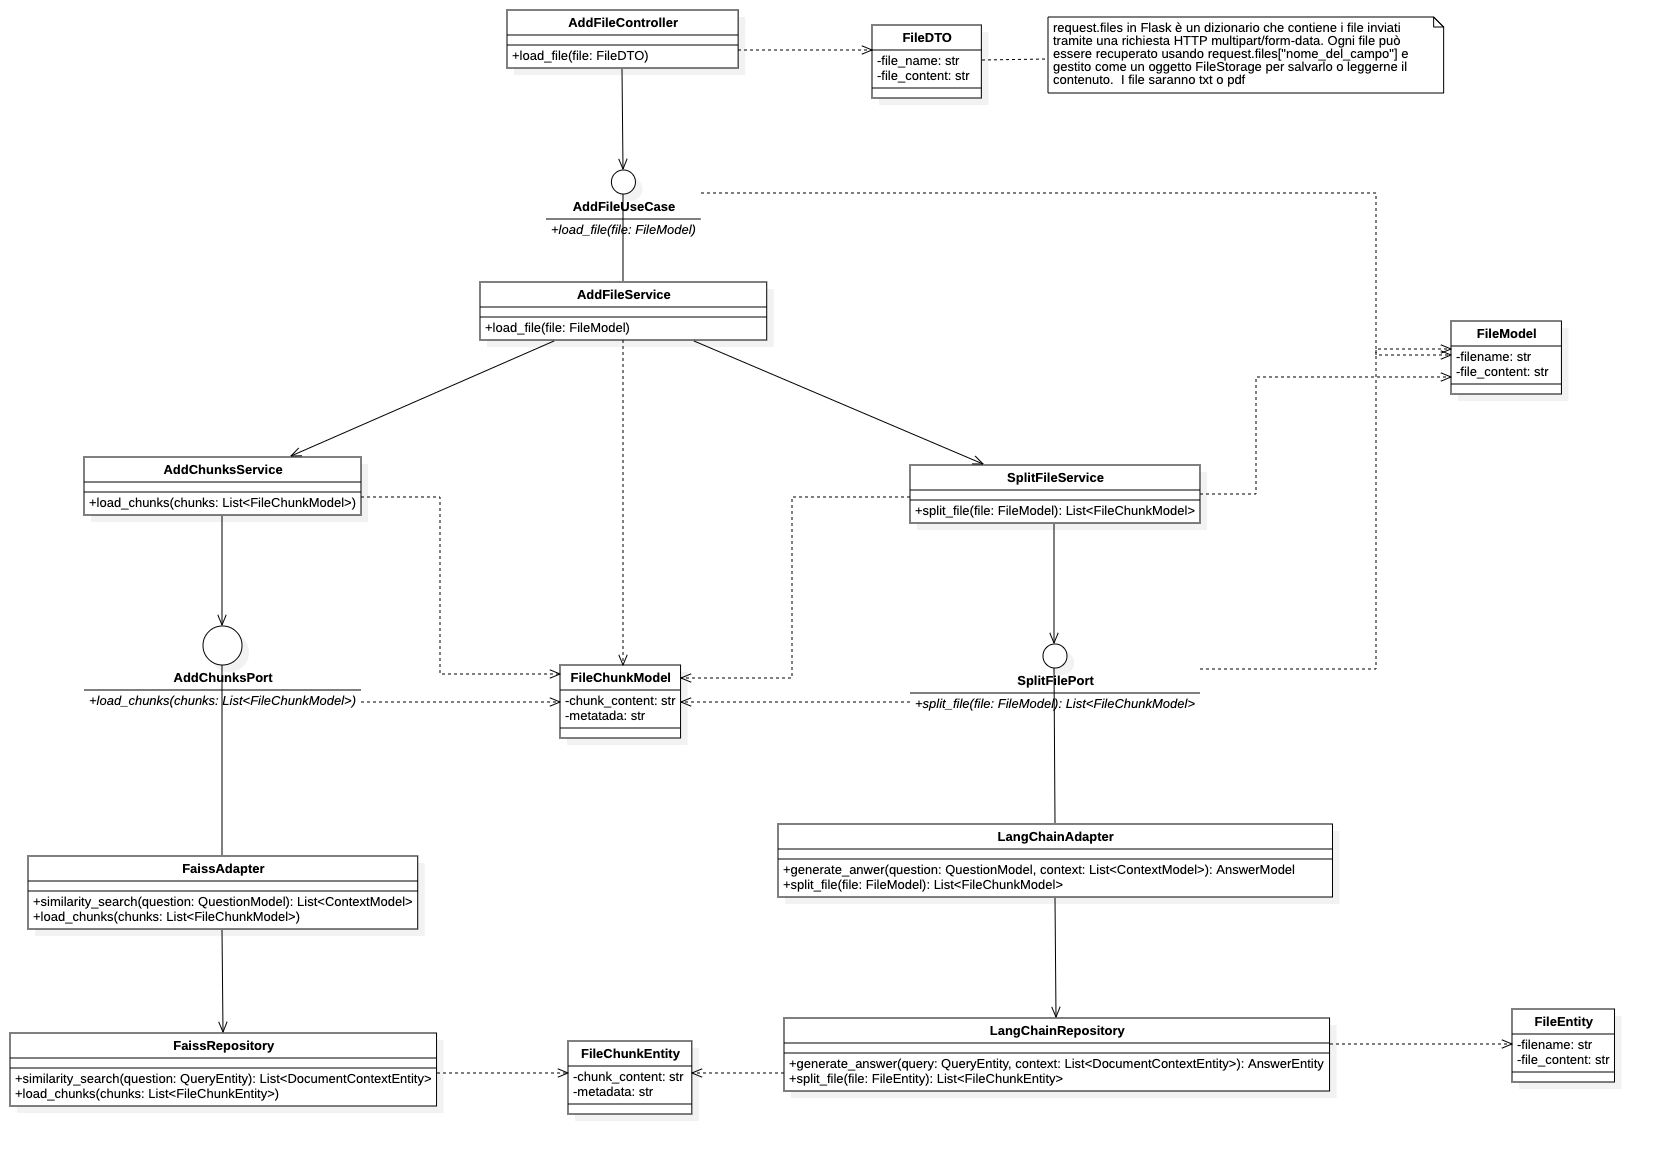
\includegraphics[width=\linewidth, height=0.8\textheight, keepaspectratio]{./img/AddFileController.png}
        \caption{Diagramma delle classi - Add File Controller}
        \label{fig:add_file_controller}
    \end{figure}

    Questo modulo implementa una struttura modulare per gestire il caricamento, il processamento e la ricerca di file (e dei loro contenuti). Di seguito viene fornita una spiegazione dettagliata dei componenti principali:

    \paragraph{1. Data Transfer Object (DTO) e Modelli di Dati}
    \begin{itemize}
        \item \textbf{FileDTO:}
        \begin{itemize}
            \item Funziona da oggetto di trasferimento dati per il file.
            \item \textbf{Attributi:}
            \begin{itemize}
                \item file\_name: Nome del file.
                \item file\_content: Contenuto del file.
            \end{itemize}
            \item \textbf{Metodi:}
            \begin{itemize}
                \item get\_file\_name(): Ritorna il nome del file.
                \item get\_file\_content(): Ritorna il contenuto del file.
            \end{itemize}
        \end{itemize}
        \item \textbf{FileModel:}
        \begin{itemize}
            \item Rappresenta il file nel dominio interno all’applicazione.
            \item \textbf{Attributi:}
            \begin{itemize}
                \item filename: Nome del file.
                \item file\_content: Contenuto del file.
            \end{itemize}
            \item \textbf{Metodi:}
            \begin{itemize}
                \item get\_filename(): Ritorna il nome del file.
                \item get\_file\_content(): Ritorna il contenuto del file.
            \end{itemize}
        \end{itemize}
        \item \textbf{FileChunkModel:}
        \begin{itemize}
            \item Modella un frammento (chunk) di file.
            \item \textbf{Attributi:}
            \begin{itemize}
                \item chunk\_content: Il contenuto del frammento.
                \item metadata: Metadati associati al frammento (ad es. informazioni sul contesto o origine).
            \end{itemize}
            \item \textbf{Metodi:}
            \begin{itemize}
                \item get\_chunk\_content(): Ritorna il contenuto del chunk.
                \item get\_metadata(): Ritorna i metadati.
            \end{itemize}
        \end{itemize}
        \item \textbf{FileEntity e FileChunkEntity:}
        \begin{itemize}
            \item \textbf{FileEntity:}
            \begin{itemize}
                \item Attributi: metadata e file\_content.
                \item Metodi: get\_metadata() e get\_file\_content().
            \end{itemize}
            \item \textbf{FileChunkEntity:}
            \begin{itemize}
                \item Attributi: chunk\_content e metadata.
                \item Metodi: get\_chunk\_content() e get\_metadata().
            \end{itemize}
        \end{itemize}
    \end{itemize}

    \paragraph{2. Controller e Use Case}
    \begin{itemize}
        \item \textbf{AddFileController:}
        \begin{itemize}
            \item \textbf{Ruolo:} Gestisce la richiesta di aggiunta di un file alla base dati.
            \item \textbf{Flusso:}
            \begin{itemize}
                \item Riceve un oggetto FileDTO.
                \item Converte il DTO in un FileModel (adattando il formato per il dominio interno).
                \item Invoca il metodo load\_file del use case associato (AddFileUseCase).
            \end{itemize}
            \item \textbf{Gestione Errori:} Nel blocco try/except, eventuali errori vengono rilanciati.
        \end{itemize}
        \item \textbf{AddFileUseCase (astratto):}
        \begin{itemize}
            \item \textbf{Scopo:} Definisce l’interfaccia per il caso d’uso di aggiunta file.
            \item \textbf{Metodo astratto:} load\_file(file: FileModel) che deve essere implementato da una classe concreta.
        \end{itemize}
    \end{itemize}

    \paragraph{3. Servizi}
    \begin{itemize}
        \item \textbf{AddFileService:}
        \begin{itemize}
            \item \textbf{Ruolo:} Gestisce la logica di business per il caricamento del file e la gestione dei suoi frammenti.
            \item \textbf{Metodi principali:}
            \begin{itemize}
                \item load\_file(file: FileModel):
                \begin{itemize}
                    \item Effettua lo split del file in frammenti (chiamando il metodo split\_file).
                    \item Carica i frammenti tramite load\_chunks.
                \end{itemize}
                \item split\_file(file: FileModel) - list[FileChunkModel]:
                \begin{itemize}
                    \item Utilizza il servizio SplitFileService per dividere il file in chunk.
                \end{itemize}
                \item load\_chunks(chunks: list[FileChunkModel]):
                \begin{itemize}
                    \item Inoltra i chunk al servizio AddChunksService.
                \end{itemize}
            \end{itemize}
        \end{itemize}
        \item \textbf{AddChunksService:}
        \begin{itemize}
            \item \textbf{Ruolo:} Si occupa del caricamento dei frammenti nel sistema di repository.
            \item \textbf{Metodo:}
            \begin{itemize}
                \item load\_chunks(chunks: list[FileChunkModel]):
                \begin{itemize}
                    \item Invoca il metodo load\_chunks del port AddChunksPort.
                \end{itemize}
            \end{itemize}
        \end{itemize}
        \item \textbf{SplitFileService:}
        \begin{itemize}
            \item \textbf{Ruolo:} Incapsula la logica per la divisione di un file in frammenti.
            \item \textbf{Metodo:}
            \begin{itemize}
                \item split\_file(file: FileModel) -> list[FileChunkModel]:
                \begin{itemize}
                    \item Delegato al port SplitFilePort.
                \end{itemize}
            \end{itemize}
        \end{itemize}
    \end{itemize}

    \paragraph{4. Port e Interfacce Astratte}
    \begin{itemize}
        \item \textbf{AddChunksPort:}
        \begin{itemize}
            \item \textbf{Scopo:} Definisce il contratto per il caricamento dei chunk in un repository (es. FAISS).
            \item \textbf{Metodo astratto:} load\_chunks(chunks: list[FileChunkModel]).
        \end{itemize}
        \item \textbf{SplitFilePort:}
        \begin{itemize}
            \item \textbf{Scopo:} Definisce il contratto per la divisione di un file in frammenti.
            \item \textbf{Metodo astratto:} split\_file(file: FileModel) -> list[FileChunkModel].
        \end{itemize}
    \end{itemize}

    \paragraph{5. Adapter e Repository}
    \begin{itemize}
        \item \textbf{FaissAdapter:}
        \begin{itemize}
            \item \textbf{Implementa:} SimilaritySearchPort e AddChunksPort.
            \item \textbf{Funzionalità:}
            \begin{itemize}
                \item Similarity Search:
                \begin{itemize}
                    \item Metodo similarity\_search(question\_model: QuestionModel):
                    \item Verifica che la domanda non sia vuota.
                    \item Crea un’entità query (QueryEntity).
                    \item Richiama il metodo similarity\_search del repository FAISS.
                    \item Trasforma i risultati in oggetti ContextModel.
                \end{itemize}
                \item Load Chunks:
                \begin{itemize}
                    \item Metodo load\_chunks(chunks: list[FileChunkModel]):
                    \item Converte i modelli in entità (FileChunkEntity) e li passa al repository FAISS.
                    \item Salva lo stato aggiornato del vector store.
                \end{itemize}
            \end{itemize}
        \end{itemize}
    \end{itemize}

    \subsubsection{Conversation}

    \begin{figure}[H]
        \centering
        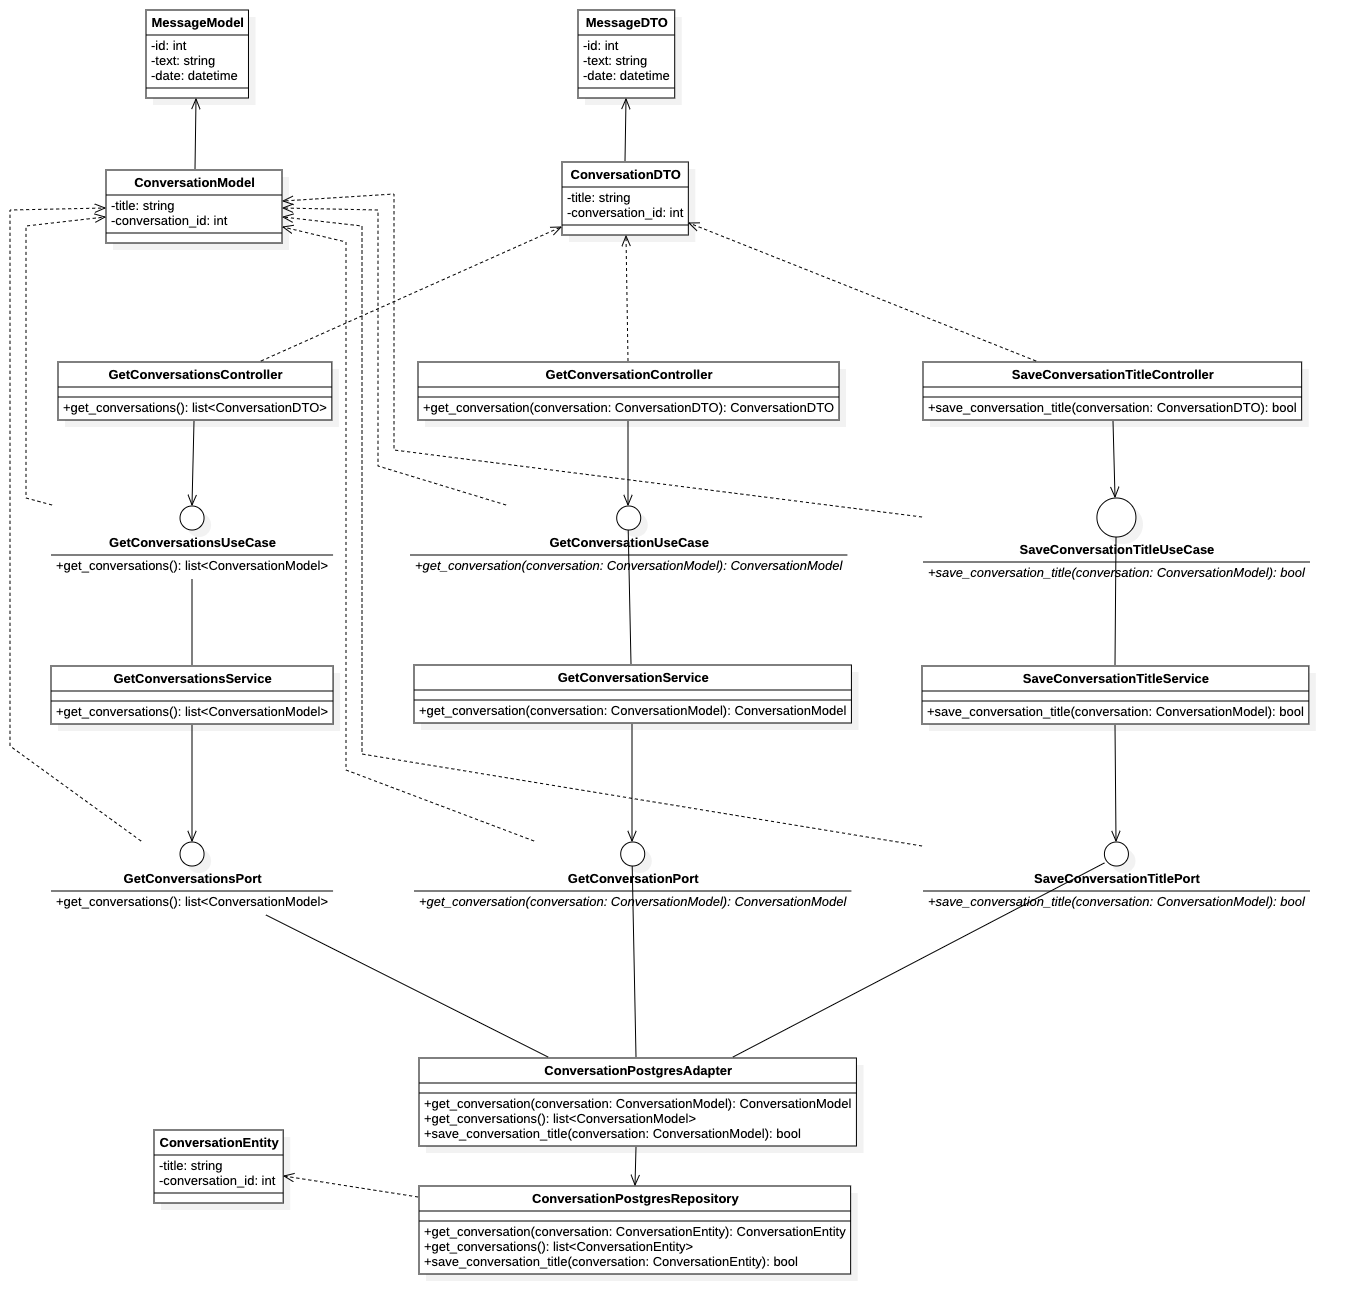
\includegraphics[width=\linewidth, height=0.8\textheight, keepaspectratio]{./img/Conversation.png}
        \caption{Diagramma delle classi - Conversation}
        \label{fig:conversation}
    \end{figure}

    Il modulo implementa un'architettura a strati (simile alla Clean Architecture) per la gestione delle conversazioni e dei messaggi in un'applicazione. Di seguito viene descritta in dettaglio la struttura e il funzionamento di ciascuna parte.

    \paragraph{1. Data Transfer Objects (DTO)}
    \begin{itemize}
        \item \textbf{MessageDTO \& ConversationDTO:}
        \begin{itemize}
            \item Questi oggetti fungono da oggetti di trasferimento dati tra i vari livelli dell'applicazione (ad esempio, tra controller e use case).
            \item \textit{MessageDTO}: Contiene attributi come id, text, is\_bot, conversation\_id, rating e created\_at.
            \item \textit{ConversationDTO}: Contiene attributi come id, title e user\_id e metodi getter per accedervi.
        \end{itemize}
    \end{itemize}

    \paragraph{2. Modelli}
    \begin{itemize}
        \item \textbf{MessageModel \& ConversationModel:}
        \begin{itemize}
            \item Questi modelli rappresentano la struttura dei dati a livello di dominio, simili ai DTO ma utilizzati internamente (per la logica di business).
            \item \textit{MessageModel}: Replicano gli attributi di MessageDTO e forniscono metodi getter per recuperarli.
            \item \textit{ConversationModel}: Replicano gli attributi di ConversationDTO e forniscono metodi getter per recuperarli.
        \end{itemize}
    \end{itemize}

    \paragraph{3. Controller}
    \begin{itemize}
        \item I controller sono responsabili della gestione delle richieste e della delega dell'elaborazione ai use case. In questo codice, sono presenti tre controller:
        \begin{itemize}
            \item \textbf{GetConversationController:}
            \begin{itemize}
                \item Riceve un oggetto ConversationDTO, lo converte in un ConversationModel e lo passa al use case \texttt{get\_conversation}.
                \item Una volta ottenuto il risultato dal use case, lo trasforma in un nuovo ConversationDTO e lo restituisce.
            \end{itemize}
            \item \textbf{GetConversationsController:}
            \begin{itemize}
                \item Lavora con una lista di conversazioni, convertendo ogni ConversationDTO in un ConversationModel.
                \item Richiama il use case per ottenere una lista di conversazioni e mappa ciascun elemento della lista in un ConversationDTO.
            \end{itemize}
            \item \textbf{SaveConversationTitleController:}
            \begin{itemize}
                \item Riceve un ConversationDTO contenente il titolo e altri dati.
                \item Converte il DTO in un model e invoca il use case \texttt{save\_conversation\_title} per salvare il titolo nel database.
                \item Restituisce l'ID della conversazione salvata.
            \end{itemize}
        \end{itemize}
    \end{itemize}

    \paragraph{4. Use Case e Interfacce Astratte}
    \begin{itemize}
        \item I use case definiscono la logica applicativa e le operazioni principali. Sono implementati tramite classi astratte che fungono da interfacce:
        \begin{itemize}
            \item \textbf{GetConversationUseCase:} Definisce il metodo astratto \texttt{get\_conversation}, che restituisce un altro ConversationModel (recuperato dal database).
            \item \textbf{GetConversationsUseCase:} Definisce il metodo astratto \texttt{get\_conversations} per ottenere una lista di conversazioni.
            \item \textbf{SaveConversationTitleUseCase:} Definisce il metodo astratto \texttt{save\_conversation\_title} per salvare il titolo di una conversazione e restituire l'ID aggiornato.
        \end{itemize}
    \end{itemize}

    \paragraph{5. Service}
    \begin{itemize}
        \item I service implementano concretamente i use case e delegano l'accesso ai dati ai cosiddetti \textit{port} (interfacce di adattamento):
        \begin{itemize}
            \item \textbf{GetConversationService:} Implementa \texttt{get\_conversation} invocando il metodo \texttt{get\_conversation} del relativo port.
            \item \textbf{GetConversationsService:} Implementa \texttt{get\_conversations} invocando il metodo \texttt{get\_conversations} del port.
            \item \textbf{SaveConversationTitleService:} Implementa \texttt{save\_conversation\_title} invocando il metodo \texttt{save\_conversation\_title} del relativo port.
        \end{itemize}
    \end{itemize}

    \paragraph{6. Ports}
    \begin{itemize}
        \item I port sono interfacce che definiscono i metodi per l'interazione con il livello di persistenza (repository). Sono definiti come classi astratte:
        \begin{itemize}
            \item \textbf{GetConversationPort:} Specifica il metodo \texttt{get\_conversation} per recuperare una conversazione.
            \item \textbf{GetConversationsPort:} Specifica il metodo \texttt{get\_conversations} per recuperare tutte le conversazioni relative a un utente.
            \item \textbf{SaveConversationTitlePort:} Specifica il metodo \texttt{save\_conversation\_title} per salvare il titolo di una conversazione.
        \end{itemize}
    \end{itemize}

    \paragraph{7. Adapter e Repository}
    \begin{itemize}
        \item \textbf{Adapter: ConversationPostgresAdapter:}
        \begin{itemize}
            \item Questa classe implementa i port (\texttt{GetConversationPort}, \texttt{GetConversationsPort}, \\ 
            \texttt{SaveConversationTitlePort}) e funge da intermediario tra il livello service e il repository.
        \end{itemize}
        \item \textbf{Repository: ConversationPostgresRepository:}
        \begin{itemize}
            \item Si occupa della comunicazione diretta con il database PostgreSQL tramite il modulo \texttt{psycopg2}.
            \item Fornisce metodi per la connessione al database, l'esecuzione di query per ottenere, salvare ed eliminare conversazioni.
        \end{itemize}
    \end{itemize}

    \paragraph{8. Flusso Complessivo}
    \begin{itemize}
        \item Ricezione della richiesta: Un controller riceve un DTO dalla parte esterna.
        \item Conversione e delega al use case: Il controller trasforma il DTO in un Model e lo passa al use case.
        \item Accesso ai dati tramite il Port: Il Service invoca il metodo del Port.
        \item Operazione sul database: L'Adapter chiama il repository per eseguire query.
        \item Restituzione della risposta: Il repository restituisce i dati all'Adapter, che li trasforma e li passa al Controller per la risposta finale.
    \end{itemize}

    \subsubsection{Message}
    \begin{figure}[H]
        \centering
        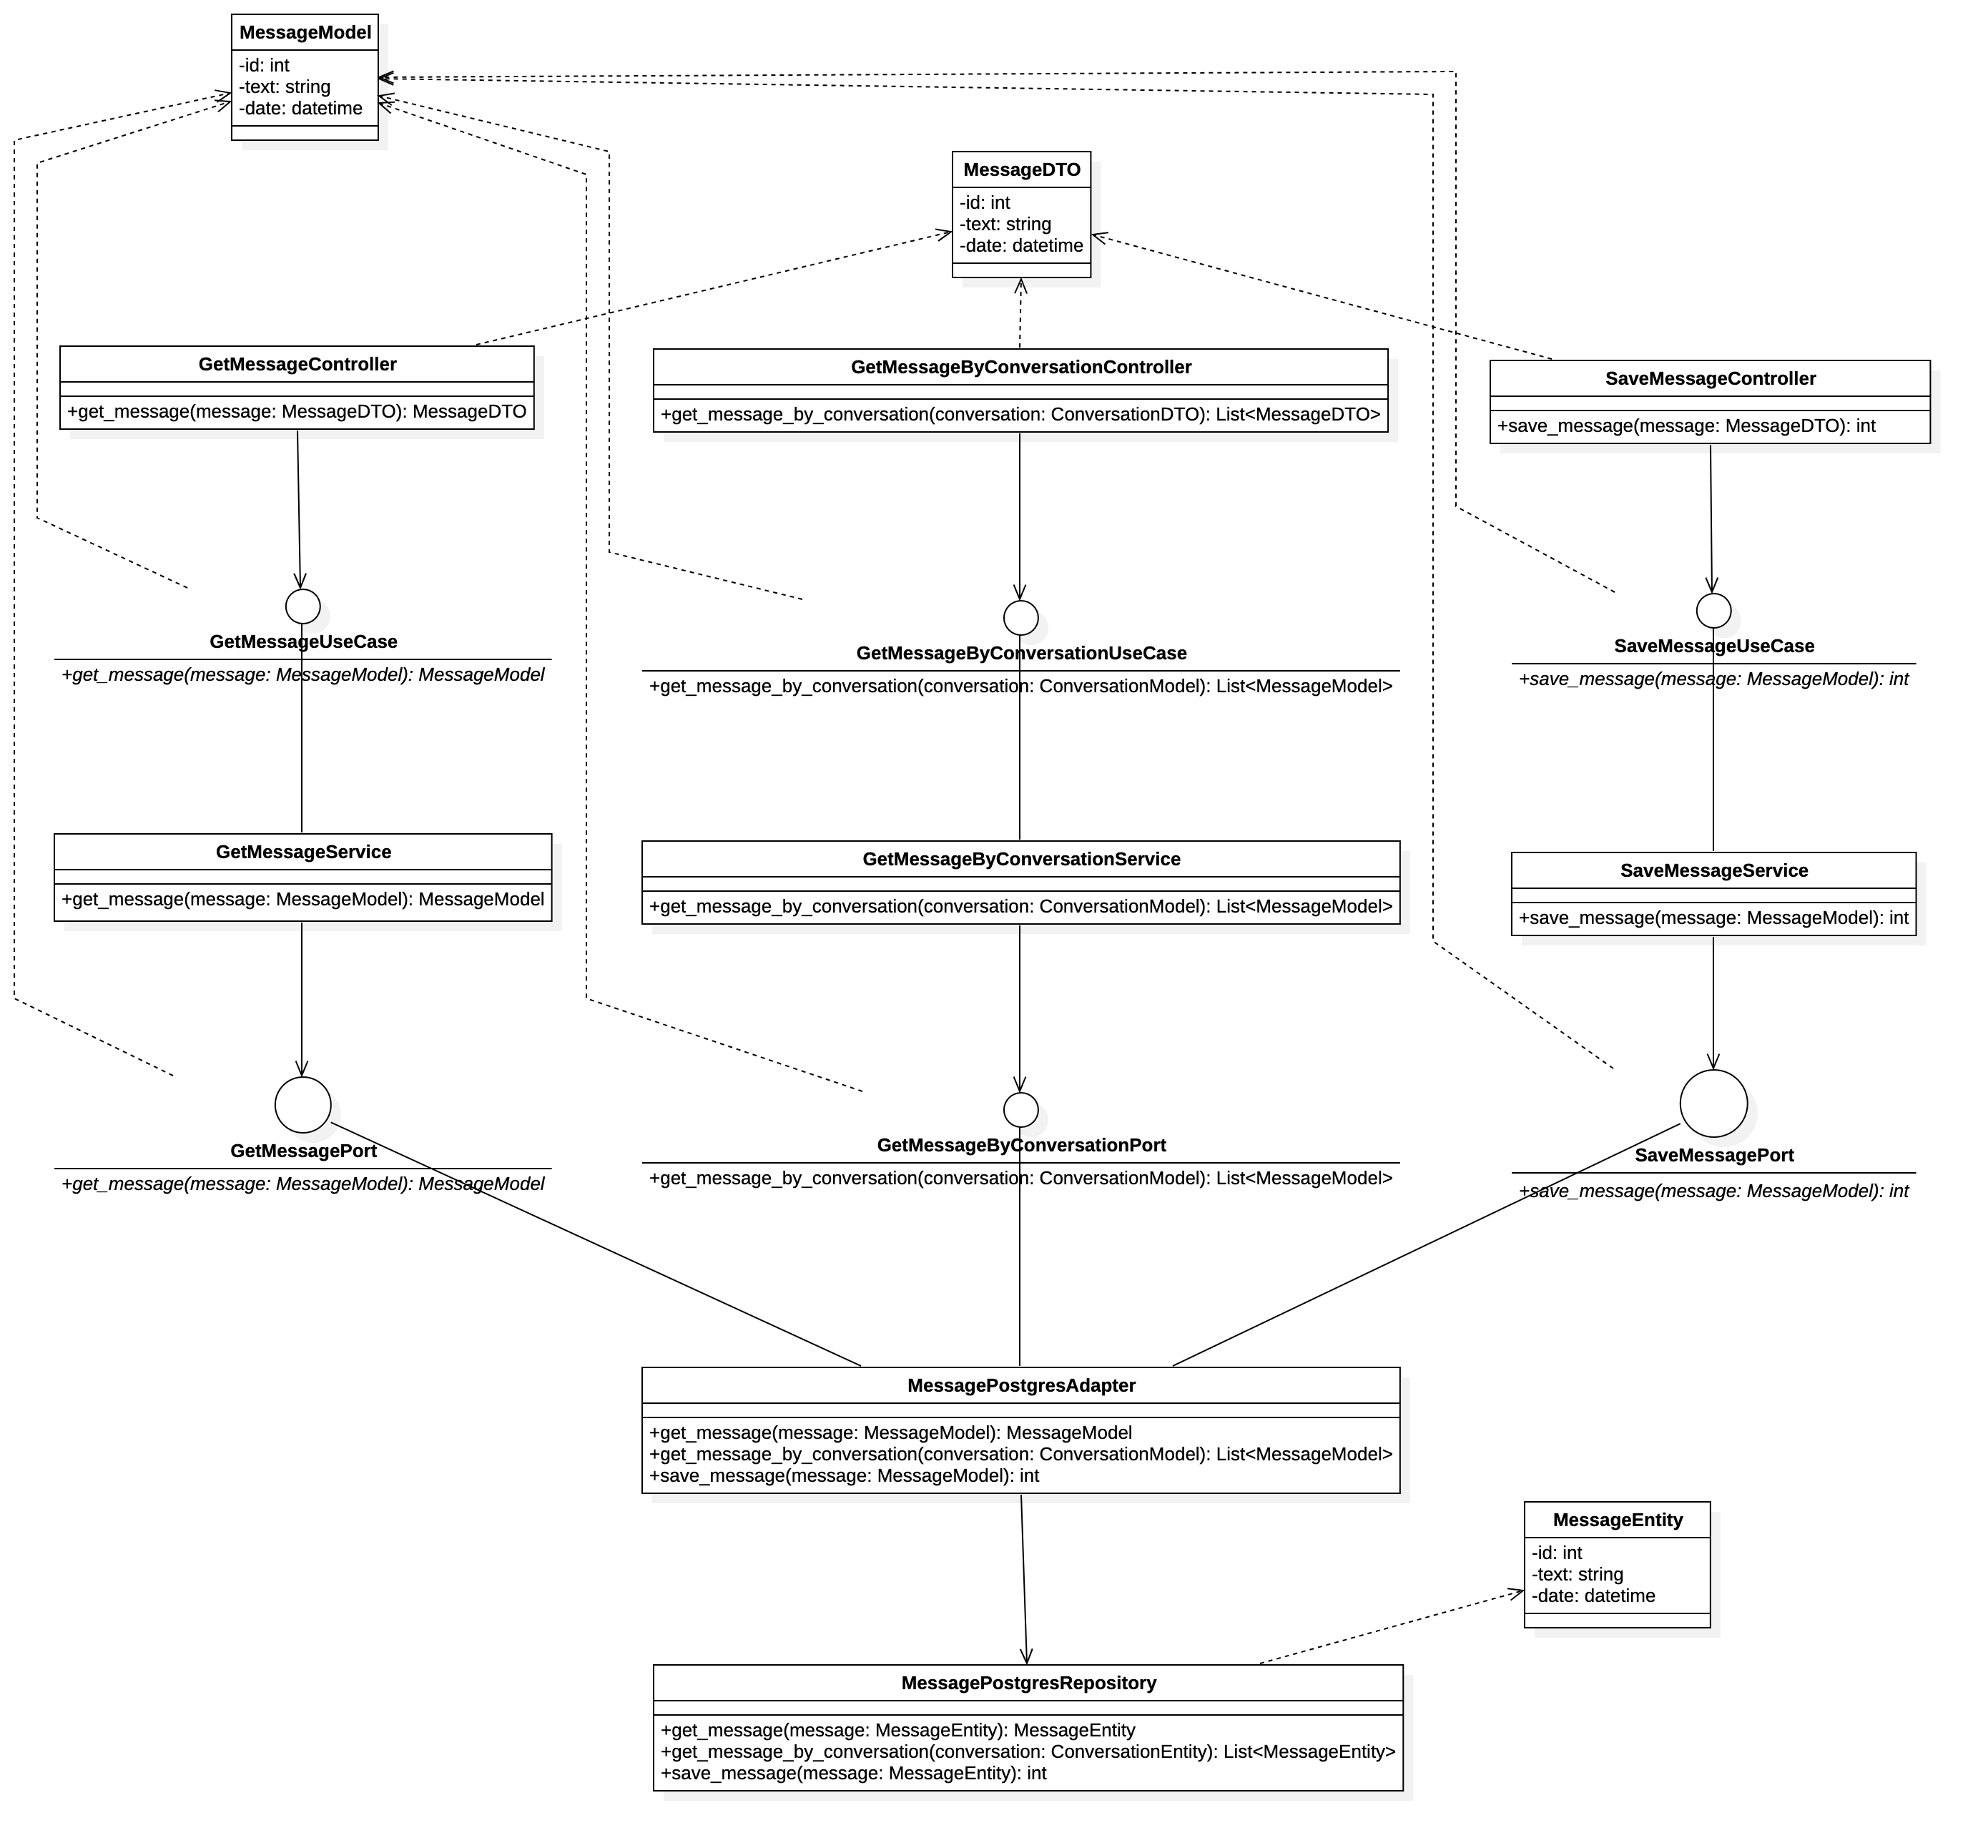
\includegraphics[width=\linewidth, height=0.8\textheight, keepaspectratio]{./img/Message.png}
        \caption{Diagramma delle classi - Message}
        \label{fig:message}
    \end{figure}

    Il modulo implementa un'architettura a più livelli per la gestione dei messaggi, separando le responsabilità in vari componenti (DTO, modelli, entità, controller, use case, servizi, porte e repository) per garantire una maggiore manutenibilità, testabilità ed estendibilità dell’applicazione. Di seguito una descrizione dettagliata dei vari componenti e del loro funzionamento:

    \paragraph{1. Data Transfer Objects (DTO), Modelli ed Entità}
    \begin{itemize}
        \item \textbf{MessageDTO:}
        \begin{itemize}
            \item È un oggetto di trasferimento dati (DTO) che incapsula le informazioni di un messaggio.
            \item \textbf{Campi:} \texttt{id}, \texttt{text}, \texttt{is\_bot}, \texttt{conversation\_id}, \texttt{rating}, \texttt{created\_at}.
            \item \textbf{Metodi Getter:} \texttt{get\_id()}, \texttt{get\_text()}, ecc.
            \item \textbf{Utilizzo:} Facilita lo scambio dei dati tra il livello di presentazione e i livelli di business/logica.
        \end{itemize}
        \item \textbf{MessageModel:}
        \begin{itemize}
            \item Rappresenta il modello di dominio per il messaggio.
            \item Ha gli stessi attributi e metodi del DTO, ma viene utilizzato all'interno della logica applicativa per eseguire operazioni, trasformazioni o validazioni.
        \end{itemize}
        \item \textbf{MessageEntity:}
        \begin{itemize}
            \item È la rappresentazione della struttura dati a livello di persistenza (database).
            \item Incapsula gli stessi dati del DTO e Model, ma viene utilizzato dal repository per interagire con il database.
        \end{itemize}
    \end{itemize}

    \paragraph{2. Controller}
    \begin{itemize}
        \item \textbf{GetMessageController:}
        \begin{itemize}
            \item Funzione: Recupera un messaggio dato il suo ID.
            \item Processo:
            \begin{enumerate}
                \item Converte il \texttt{MessageDTO} ricevuto in un \texttt{MessageModel}.
                \item Chiama il metodo \texttt{get\_message} del relativo use case.
                \item Se il messaggio viene trovato, viene convertito nuovamente in un \texttt{MessageDTO}.
            \end{enumerate}
            \item Error Handling: Gestisce eventuali eccezioni rilanciate.
        \end{itemize}
        \item \textbf{GetMessagesByConversationController:}
        \begin{itemize}
            \item Funzione: Recupera tutti i messaggi relativi ad una specifica conversazione.
            \item Processo:
            \begin{enumerate}
                \item Converte il DTO della conversazione in un modello.
                \item Invoca il metodo \texttt{get\_messages\_by\_conversation} del use case.
                \item Crea un nuovo \texttt{MessageDTO} per ogni modello restituito e restituisce la lista.
            \end{enumerate}
            \item Error Handling: Rilancia eventuali eccezioni.
        \end{itemize}
        \item \textbf{SaveMessageController:}
        \begin{itemize}
            \item Funzione: Salva un nuovo messaggio nel database.
            \item Processo:
            \begin{enumerate}
                \item Converte il \texttt{MessageDTO} in un \texttt{MessageModel}.
                \item Chiama il metodo \texttt{save\_message} del use case.
                \item Restituisce l’ID del messaggio salvato.
            \end{enumerate}
            \item Error Handling: Gestisce le eccezioni.
        \end{itemize}
    \end{itemize}

    \paragraph{3. Use Case (Interfacce astratte e Implementazioni di servizio)}
    \begin{itemize}
        \item \textbf{GetMessageUseCase:}
        \begin{itemize}
            \item Definisce il metodo \texttt{get\_message} che, dato un \texttt{MessageModel}, restituisce il messaggio corrispondente.
        \end{itemize}
        \item \textbf{GetMessagesByConversationUseCase:}
        \begin{itemize}
            \item Definisce il metodo \texttt{get\_messages\_by\_conversation} per ottenere una lista di messaggi di una conversazione.
        \end{itemize}
        \item \textbf{SaveMessageUseCase:}
        \begin{itemize}
            \item Definisce il metodo \texttt{save\_message} per salvare un messaggio e restituire l'ID.
        \end{itemize}
    \end{itemize}

    \paragraph{4. Porte (Interfaces) e Adapter}
    \begin{itemize}
        \item \textbf{GetMessagePort, GetMessagesByConversationPort, SaveMessagePort:}
        \begin{itemize}
            \item Ogni interfaccia espone il metodo necessario per eseguire l’operazione di recupero o salvataggio.
            \item Queste interfacce sono implementate da un adattatore concreto.
        \end{itemize}
        \item \textbf{MessagePostgresAdapter:}
        \begin{itemize}
            \item \textbf{Funzioni principali:}
            \begin{enumerate}
                \item \texttt{get\_message}: Converte un \texttt{MessageModel} in \texttt{MessageEntity} e richiama il metodo \texttt{get\_message} del repository.
                \item \texttt{get\_messages\_by\_conversation}: Converte l’input in una \texttt{MessageEntity} e invoca il repository per ottenere la lista di messaggi.
                \item \texttt{save\_message}: Converte il \texttt{MessageModel} in un \texttt{MessageEntity}, invoca il repository per il salvataggio e restituisce l’ID.
            \end{enumerate}
        \end{itemize}
    \end{itemize}

    \paragraph{5. Repository}
    \begin{itemize}
        \item \textbf{MessagePostgresRepository:}
        \begin{itemize}
            \item \textbf{\_\_init\_\_}: Inizializza il repository con una configurazione del database.
            \item \textbf{\_\_connect}: Crea una connessione al database.
            \item \texttt{get\_message}: Esegue una query per recuperare un messaggio in base all’ID.
            \item \texttt{get\_messages\_by\_conversation}: Esegue una query per ottenere tutti i messaggi di una conversazione.
            \item \texttt{save\_message}: Inserisce un messaggio nel database e restituisce l'ID.
            \item \texttt{delete\_message}: (opzionale) Cancella un messaggio dato l'ID.
        \end{itemize}
    \end{itemize}

    \paragraph{6. Integrazione e Flusso Complessivo}
    \begin{itemize}
        \item Il flusso per salvare o recuperare un messaggio è il seguente:
        \begin{enumerate}
            \item Il controller riceve un \texttt{MessageDTO}.
            \item Converte il DTO in un \texttt{MessageModel}.
            \item Chiama il metodo appropriato del use case.
            \item Il use case delega la richiesta alla porta (ad esempio, \texttt{MessagePostgresAdapter}).
            \item La porta chiama il repository per eseguire l'operazione sul database.
            \item I dati vengono ritrasformati fino a essere restituiti come \texttt{MessageDTO}.
        \end{enumerate}
    \end{itemize}

    \subsubsection{User}

    \begin{figure}[H]
        \centering
        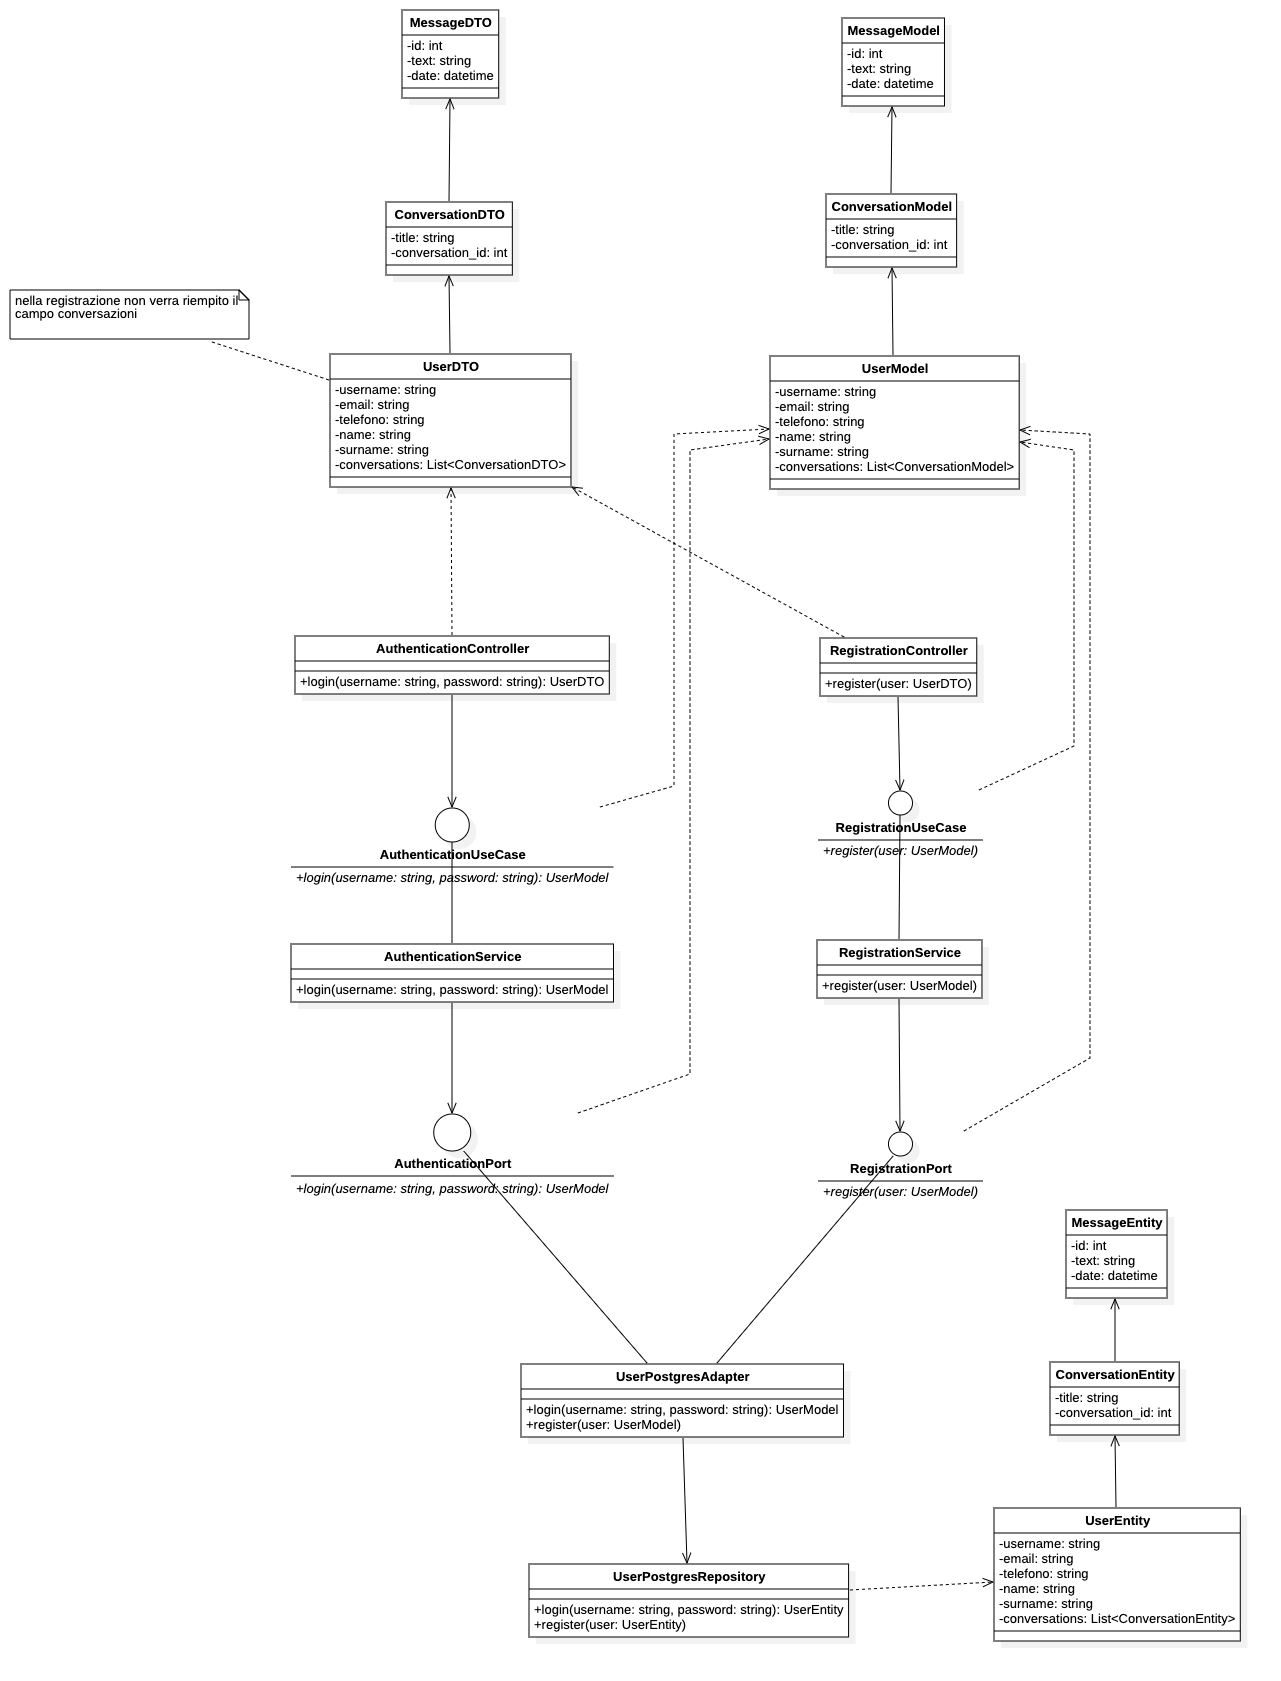
\includegraphics[width=\linewidth, height=0.8\textheight, keepaspectratio]{./img/User.png}
        \caption{Diagramma delle classi - User}
        \label{fig:user}
    \end{figure}

    \paragraph{1. Data Transfer Objects (DTO)}
    \begin{itemize}
        \item \textbf{MessageDTO:}
        \begin{itemize}
            \item Rappresenta un messaggio in una conversazione.
            \item Attributi: \texttt{id}, \texttt{text}, \texttt{is\_bot}, \texttt{conversation\_id}, \texttt{rating}, \texttt{created\_at}.
            \item Ha metodi getter per recuperare i valori.
        \end{itemize}
        \item \textbf{ConversationDTO:}
        \begin{itemize}
            \item Rappresenta una conversazione.
            \item Attributi: \texttt{id}, \texttt{title}, \texttt{user\_id}.
            \item Ha metodi getter.
        \end{itemize}
        \item \textbf{UserDTO:}
        \begin{itemize}
            \item Rappresenta un utente.
            \item Attributi: \texttt{id}, \texttt{username}, \texttt{password}, \texttt{email}, \texttt{phone}, \texttt{first\_name}, \texttt{last\_name}, \texttt{is\_admin}.
            \item Ha metodi getter e \texttt{set\_password} per modificare la password.
        \end{itemize}
    \end{itemize}

    \paragraph{2. Modelli e Entità}
    \begin{itemize}
        \item \textbf{MessageModel:}
        \begin{itemize}
            \item Stessi attributi del \texttt{MessageDTO}.
            \item Metodi getter per ottenere i valori.
        \end{itemize}
        \item \textbf{ConversationModel:}
        \begin{itemize}
            \item Stessi attributi di \texttt{ConversationDTO}.
        \end{itemize}
        \item \textbf{UserModel:}
        \begin{itemize}
            \item Stessi attributi di \texttt{UserDTO}.
            \item Contiene un metodo \texttt{set\_password} per aggiornare la password.
        \end{itemize}
    \end{itemize}

    \paragraph{3. Entità}
    \begin{itemize}
        \item \textbf{MessageEntity, ConversationEntity, UserEntity:}
        \begin{itemize}
            \item Stessi attributi delle corrispondenti classi Model e DTO.
        \end{itemize}
    \end{itemize}

    \paragraph{4. Controller}
    \begin{itemize}
        \item \textbf{AuthenticationController:}
        \begin{itemize}
            \item Metodo \texttt{login(user\_dto: UserDTO) -> UserDTO}.
            \item Converte \texttt{UserDTO} in \texttt{UserModel}.
            \item Chiama \texttt{authentication\_use\_case.login(user\_model)}.
            \item Restituisce un \texttt{UserDTO} basato sull'output.
        \end{itemize}
        \item \textbf{RegistrationController:}
        \begin{itemize}
            \item Metodo \texttt{register(user\_dto: UserDTO) -> bool}.
            \item Converte \texttt{UserDTO} in \texttt{UserModel}.
            \item Chiama \texttt{registration\_use\_case.register(user\_model)}.
            \item Restituisce \texttt{True} o \texttt{False}.
        \end{itemize}
    \end{itemize}

    \paragraph{5. Use Case}
    \begin{itemize}
        \item \textbf{AuthenticationUseCase:}
        \begin{itemize}
            \item Metodo \texttt{login(user\_model: UserModel) -> UserModel} (non implementato).
        \end{itemize}
        \item \textbf{RegistrationUseCase:}
        \begin{itemize}
            \item Metodo \texttt{register(user\_model: UserModel) -> bool} (non implementato).
        \end{itemize}
    \end{itemize}

    \paragraph{6. Servizi}
    \begin{itemize}
        \item \textbf{AuthenticationService:}
        \begin{itemize}
            \item Implementa \texttt{login(user\_model: UserModel) -> UserModel}.
            \item Recupera l'utente dal database tramite \\
                \texttt{authentication\_port.get\_user\_for\_authentication(user\_model)}.
            \item Controlla la validità della password con \texttt{bcrypt.check\_password\_hash}.
            \item Se tutto è corretto, restituisce l'utente autenticato.
        \end{itemize}
        \item \textbf{RegistrationService:}
        \begin{itemize}
            \item Implementa \texttt{register(user\_model: UserModel) -> bool}.
            \item Valida i dati dell'utente.
            \item Hash della password con \texttt{bcrypt.generate\_password\_hash}.
            \item Registra l'utente nel database tramite \texttt{registration\_port.register(user\_model)}.
        \end{itemize}
    \end{itemize}

    \paragraph{7. Ports}
    \begin{itemize}
        \item \textbf{AuthenticationPort:}
        \begin{itemize}
            \item Definisce \texttt{get\_user\_for\_authentication(user\_model: UserModel) -> UserModel}.
        \end{itemize}
        \item \textbf{RegistrationPort:}
        \begin{itemize}
            \item Definisce \texttt{register(user\_model: UserModel) -> bool}.
        \end{itemize}
    \end{itemize}

    \paragraph{8. Repository}
    \begin{itemize}
        \item \textbf{UserPostgresRepository:}
        \begin{itemize}
            \item Usa \texttt{psycopg2} per connettersi a PostgreSQL.
            \item \texttt{register(user\_model: UserEntity) -> bool}.
            \item Esegue \texttt{INSERT INTO Users (\dots) VALUES (\dots)} per salvare l'utente.
            \item \texttt{get\_user\_by\_email(email: str) -> bool}.
            \item Controlla se un utente con una determinata email esiste nel database.
            \item \texttt{get\_user\_by\_username(username: str) -> bool}.
            \item Controlla se un utente con un determinato username esiste.
            \item \texttt{get\_user\_for\_authentication(user: UserEntity) -> UserEntity}.
            \item Recupera un utente per il login in base all'username.
        \end{itemize}
    \end{itemize}

    \paragraph{9. Adattatori (Adapters)}
    \begin{itemize}
        \item \textbf{UserPostgresAdapter:}
        \begin{itemize}
            \item Implementa le interfacce \texttt{RegistrationPort}, \texttt{ValidationPort}, \texttt{AuthenticationPort}.
            \item Converte \texttt{UserModel} in \texttt{UserEntity} prima di chiamare il repository.
            \item Fornisce i metodi:
            \begin{itemize}
                \item \texttt{register(user\_model: UserModel) -> bool}.
                \item \texttt{get\_user\_by\_email(email: str) -> bool}.
                \item \texttt{get\_user\_by\_username(username: str) -> bool}.
                \item \texttt{get\_user\_for\_authentication(user\_model: UserModel) -> UserModel}.
            \end{itemize}
        \end{itemize}
    \end{itemize}

    \subsubsection{Support Message}

    \begin{figure}[H]
        \centering
        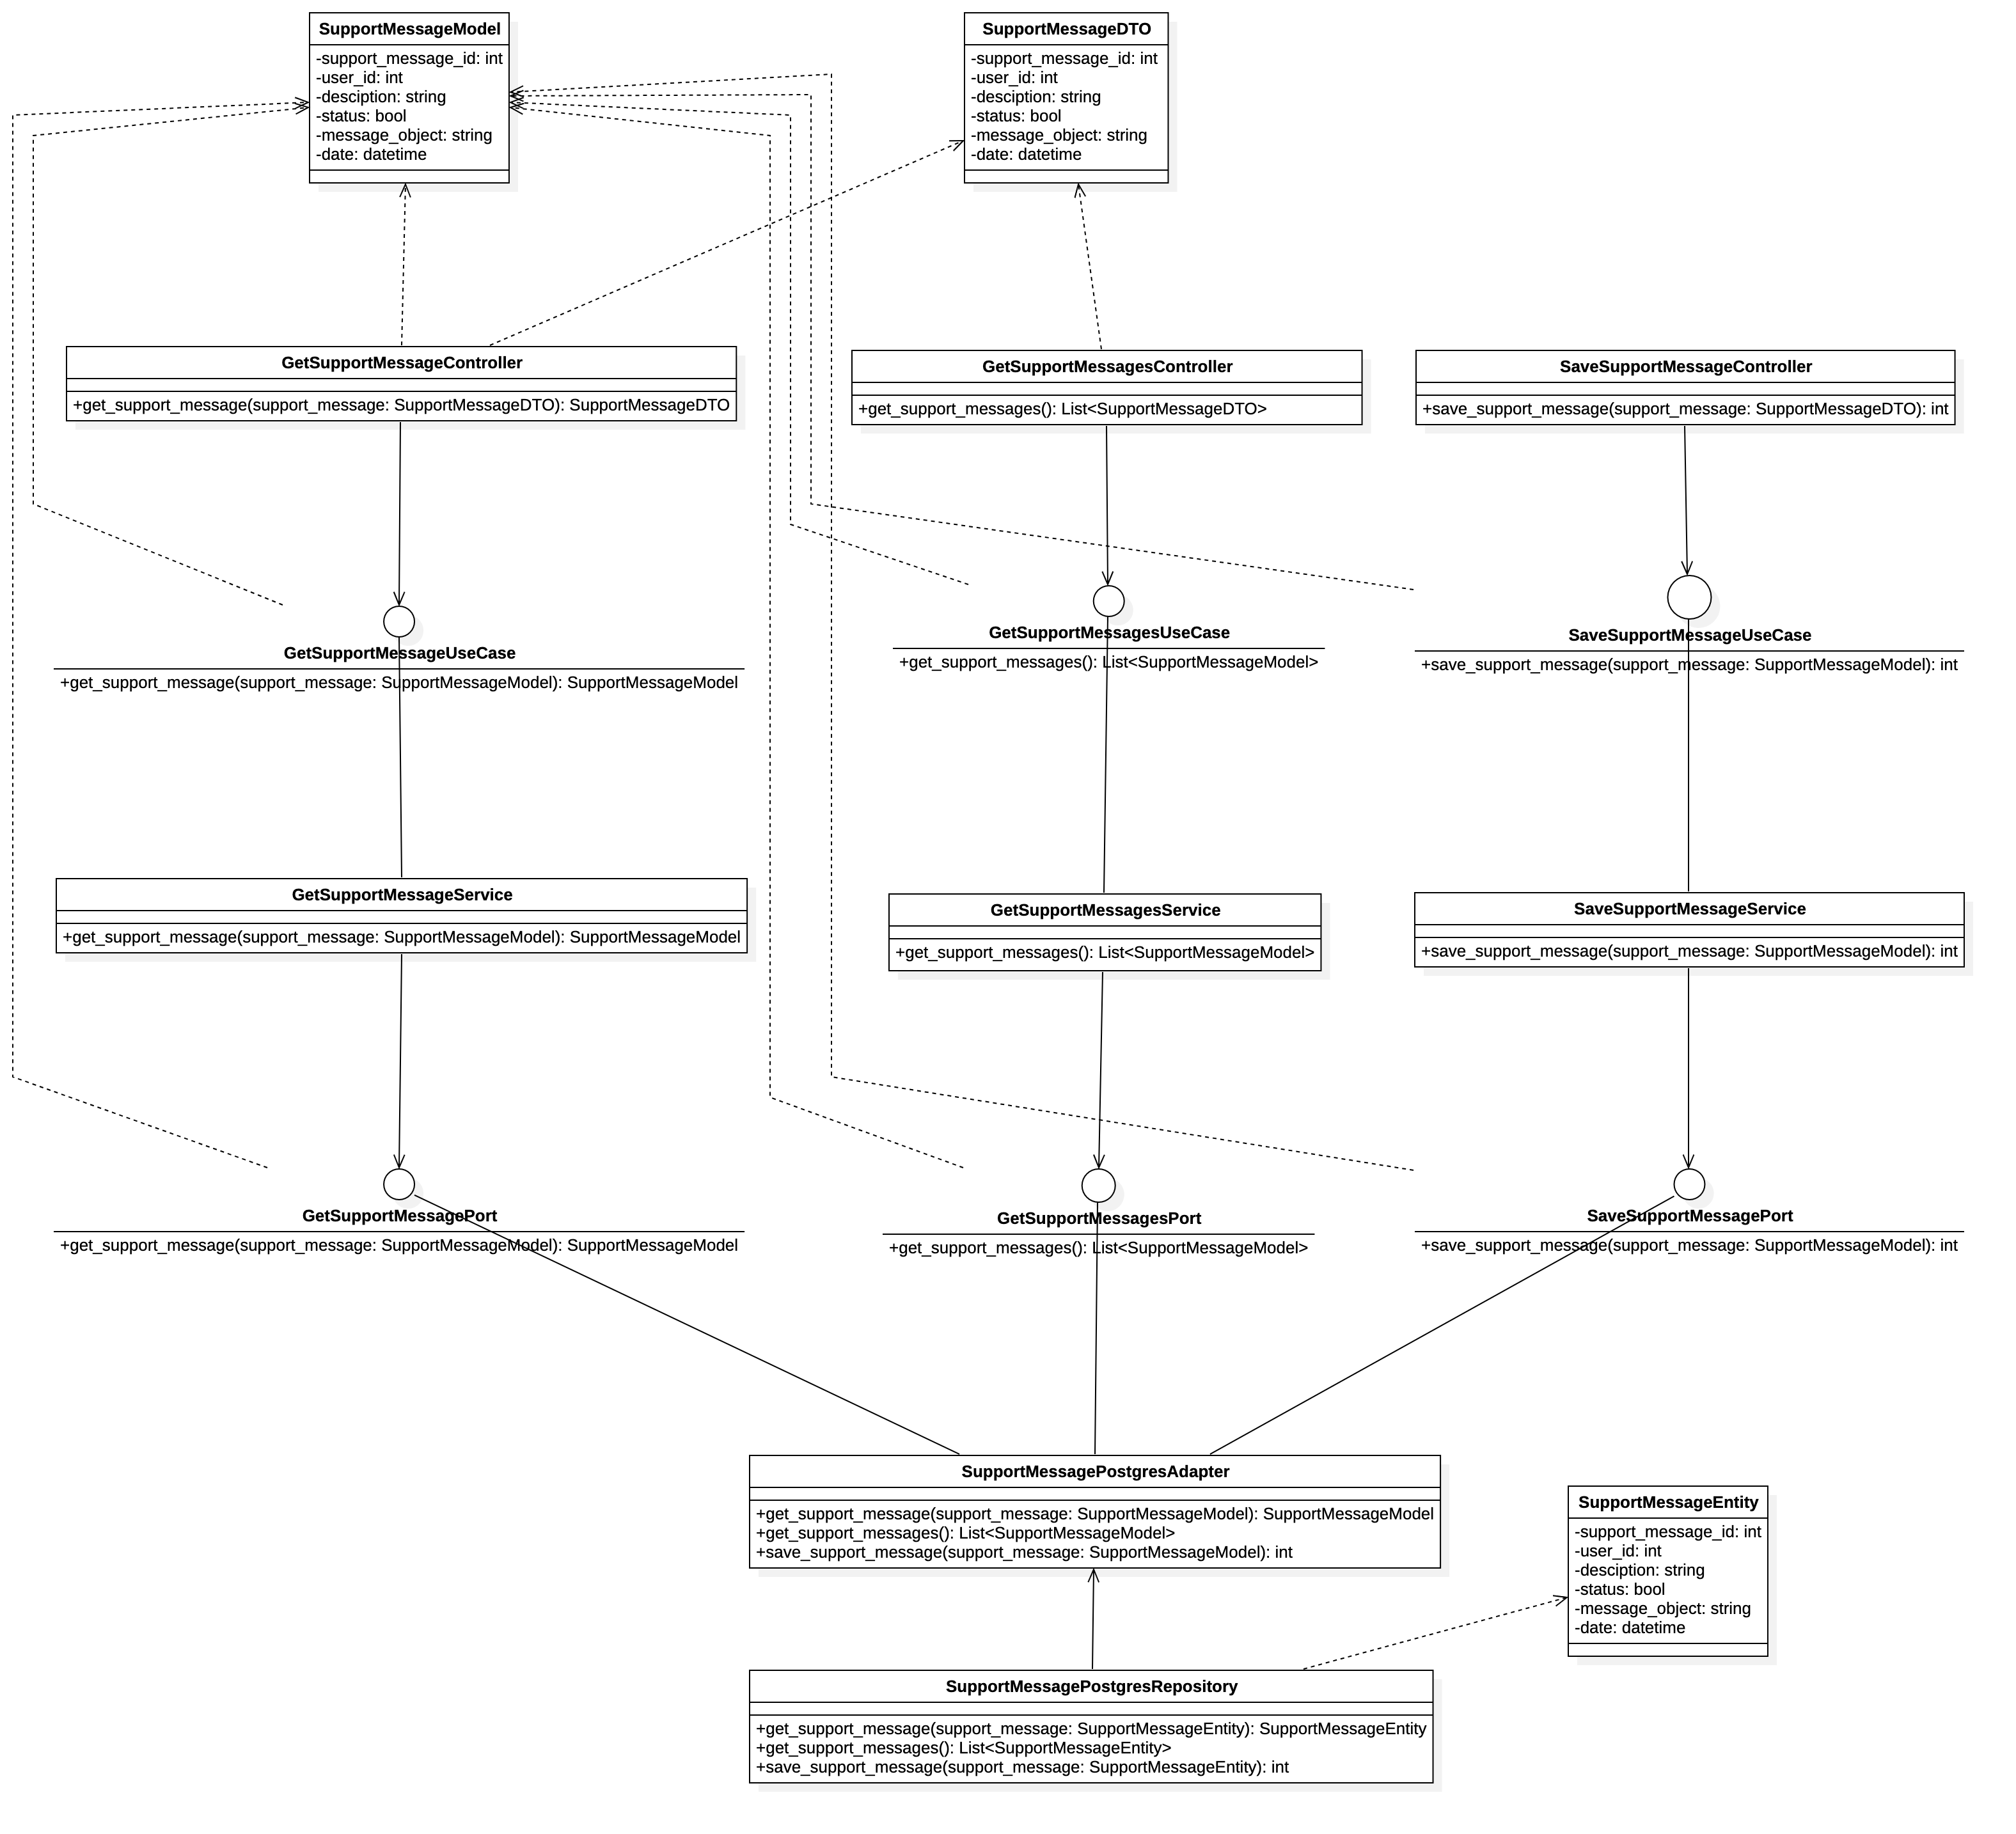
\includegraphics[width=\linewidth, height=0.8\textheight, keepaspectratio]{./img/SupportMessage.png}
        \caption{Diagramma delle classi - Support Message}
        \label{fig:support_message}
    \end{figure}

    \paragraph{1. Data Transfer Objects (DTO)}
    \begin{itemize}
        \item \textbf{SupportMessageDTO:}
        \begin{itemize}
            \item \textit{Scopo:} Funziona da Data Transfer Object, utilizzato per trasportare i dati tra i vari strati dell’applicazione (ad esempio, dal controller al service o viceversa).
            \item \textit{Attributi:} id, user\_id, description, status, subject, created\_at.
            \item \textit{Metodi:} Getter per ciascun attributo (ad esempio, get\_id(), get\_user\_id(), ecc.).
            \item \textit{Utilizzo:} Incapsula i dati di un messaggio di supporto e li trasporta tra le componenti dell’applicazione senza esporre direttamente le strutture interne.
        \end{itemize}
    \end{itemize}

    \paragraph{2. Modelli ed Entità}
    \begin{itemize}
        \item \textbf{SupportMessageModel:}
        \begin{itemize}
            \item \textit{Scopo:} Rappresenta il modello di dominio del messaggio di supporto.
            \item \textit{Caratteristiche:} Struttura simile al DTO, con gli stessi attributi e getter.
            \item \textit{Utilizzo:} Utilizzato nei casi d’uso e nei servizi per manipolare i dati secondo la logica applicativa, mantenendo separazione tra livello di presentazione (DTO) e logica di business (Model).
        \end{itemize}
        \item \textbf{SupportMessageEntity:}
        \begin{itemize}
            \item \textit{Scopo:} Rappresenta l’entità come viene memorizzata nel database.
            \item \textit{Caratteristiche:} Struttura e metodi (getter) simili a DTO e Model.
            \item \textit{Utilizzo:} Utilizzata per l’accesso al database, convertendo i dati da modello a entità e viceversa.
        \end{itemize}
    \end{itemize}

    \paragraph{3. Controller}
    \begin{itemize}
        \item \textbf{GetSupportMessageController:}
        \begin{itemize}
            \item \textit{Funzione:} Recupera un singolo messaggio di supporto.
            \item \textit{Processo:}
            \begin{enumerate}
                \item Riceve un SupportMessageDTO.
                \item Converte il DTO in un SupportMessageModel.
                \item Invoca il metodo get\_support\_message del caso d’uso.
                \item Se il risultato esiste, converte il modello ritornato nuovamente in DTO e lo restituisce.
                \item Gestisce eventuali eccezioni.
            \end{enumerate}
        \end{itemize}
        \item \textbf{GetSupportMessagesController:}
        \begin{itemize}
            \item \textit{Funzione:} Recupera tutti i messaggi di supporto.
            \item \textit{Processo:}
            \begin{enumerate}
                \item Chiama il caso d’uso per ottenere una lista di modelli.
                \item Converte ciascun modello in un SupportMessageDTO.
                \item Restituisce una lista di DTO.
            \end{enumerate}
        \end{itemize}
        \item \textbf{SaveSupportMessageController:}
        \begin{itemize}
            \item \textit{Funzione:} Salva un nuovo messaggio di supporto.
            \item \textit{Processo:}
            \begin{enumerate}
                \item Riceve un DTO in ingresso.
                \item Lo converte in un SupportMessageModel.
                \item Chiama il caso d’uso per salvare il messaggio.
                \item Ritorna l’ID del messaggio salvato.
            \end{enumerate}
        \end{itemize}
    \end{itemize}

    \paragraph{4. Use Case e Service}
    \begin{itemize}
        \item \textbf{Interfacce (Use Cases):}
        \begin{itemize}
            \item \textit{GetSupportMessageUseCase, GetSupportMessagesUseCase, SaveSupportMessageUseCase:} Definiscono in modo astratto le operazioni principali (ottenere un messaggio, ottenere tutti i messaggi, salvare un messaggio). Sono classi astratte che impongono la definizione dei metodi necessari.
        \end{itemize}
        \item \textbf{Implementazioni (Service):}
        \begin{itemize}
            \item \textit{GetSupportMessageService, GetSupportMessagesService, SaveSupportMessageService:} Implementano le interfacce sopra menzionate.
            \item Agiscono come “service layer” invocando i metodi definiti nei port (interfacce per l’accesso ai dati) e incapsulando la logica di business.
            \item Utilizzano blocchi try/except per gestire eventuali eccezioni e garantire una propagazione controllata degli errori.
        \end{itemize}
    \end{itemize}

    \paragraph{5. Port e Adapter}
    \begin{itemize}
        \item \textbf{Port:}
        \begin{itemize}
            \item \textit{Definizione:} I “port” sono interfacce (ad esempio, GetSupportMessagePort, GetSupportMessagesPort, SaveSupportMessagePort) che definiscono il contratto per l’accesso ai dati.
            \item Permettono l’astrazione rispetto al mezzo di persistenza (database, API, ecc.), rendendo l’applicazione indipendente dalla tecnologia usata per il salvataggio o il recupero dei dati.
        \end{itemize}
        \item \textbf{Adapter:}
        \begin{itemize}
            \item \textit{SupportMessagePostgresAdapter:} Implementa i port sopra citati per ottenere e salvare i messaggi di supporto. Converte tra SupportMessageModel e SupportMessageEntity, garantendo la corretta interazione con il repository.
        \end{itemize}
    \end{itemize}

    \paragraph{6. Repository per PostgreSQL}
    \begin{itemize}
        \item \textbf{MessagePostgresRepository:}
        \begin{itemize}
            \item \textit{Scopo:} Fornisce l’accesso diretto al database PostgreSQL utilizzando la libreria psycopg2.
            \item \textit{Metodi principali:}
            \begin{itemize}
                \item \_\_connect: Metodo privato per stabilire la connessione al database.
                \item get\_message: Recupera un singolo messaggio basandosi sull’ID.
                \item get\_messages\_by\_conversation: Recupera tutti i messaggi relativi a una conversazione.
                \item save\_message: Inserisce un nuovo messaggio nel database e restituisce l’ID generato.
                \item delete\_message: Elimina un messaggio dal database.
            \end{itemize}
        \end{itemize}
    \end{itemize}

    \subsubsection{Template}

    \begin{figure}[H]
        \centering
        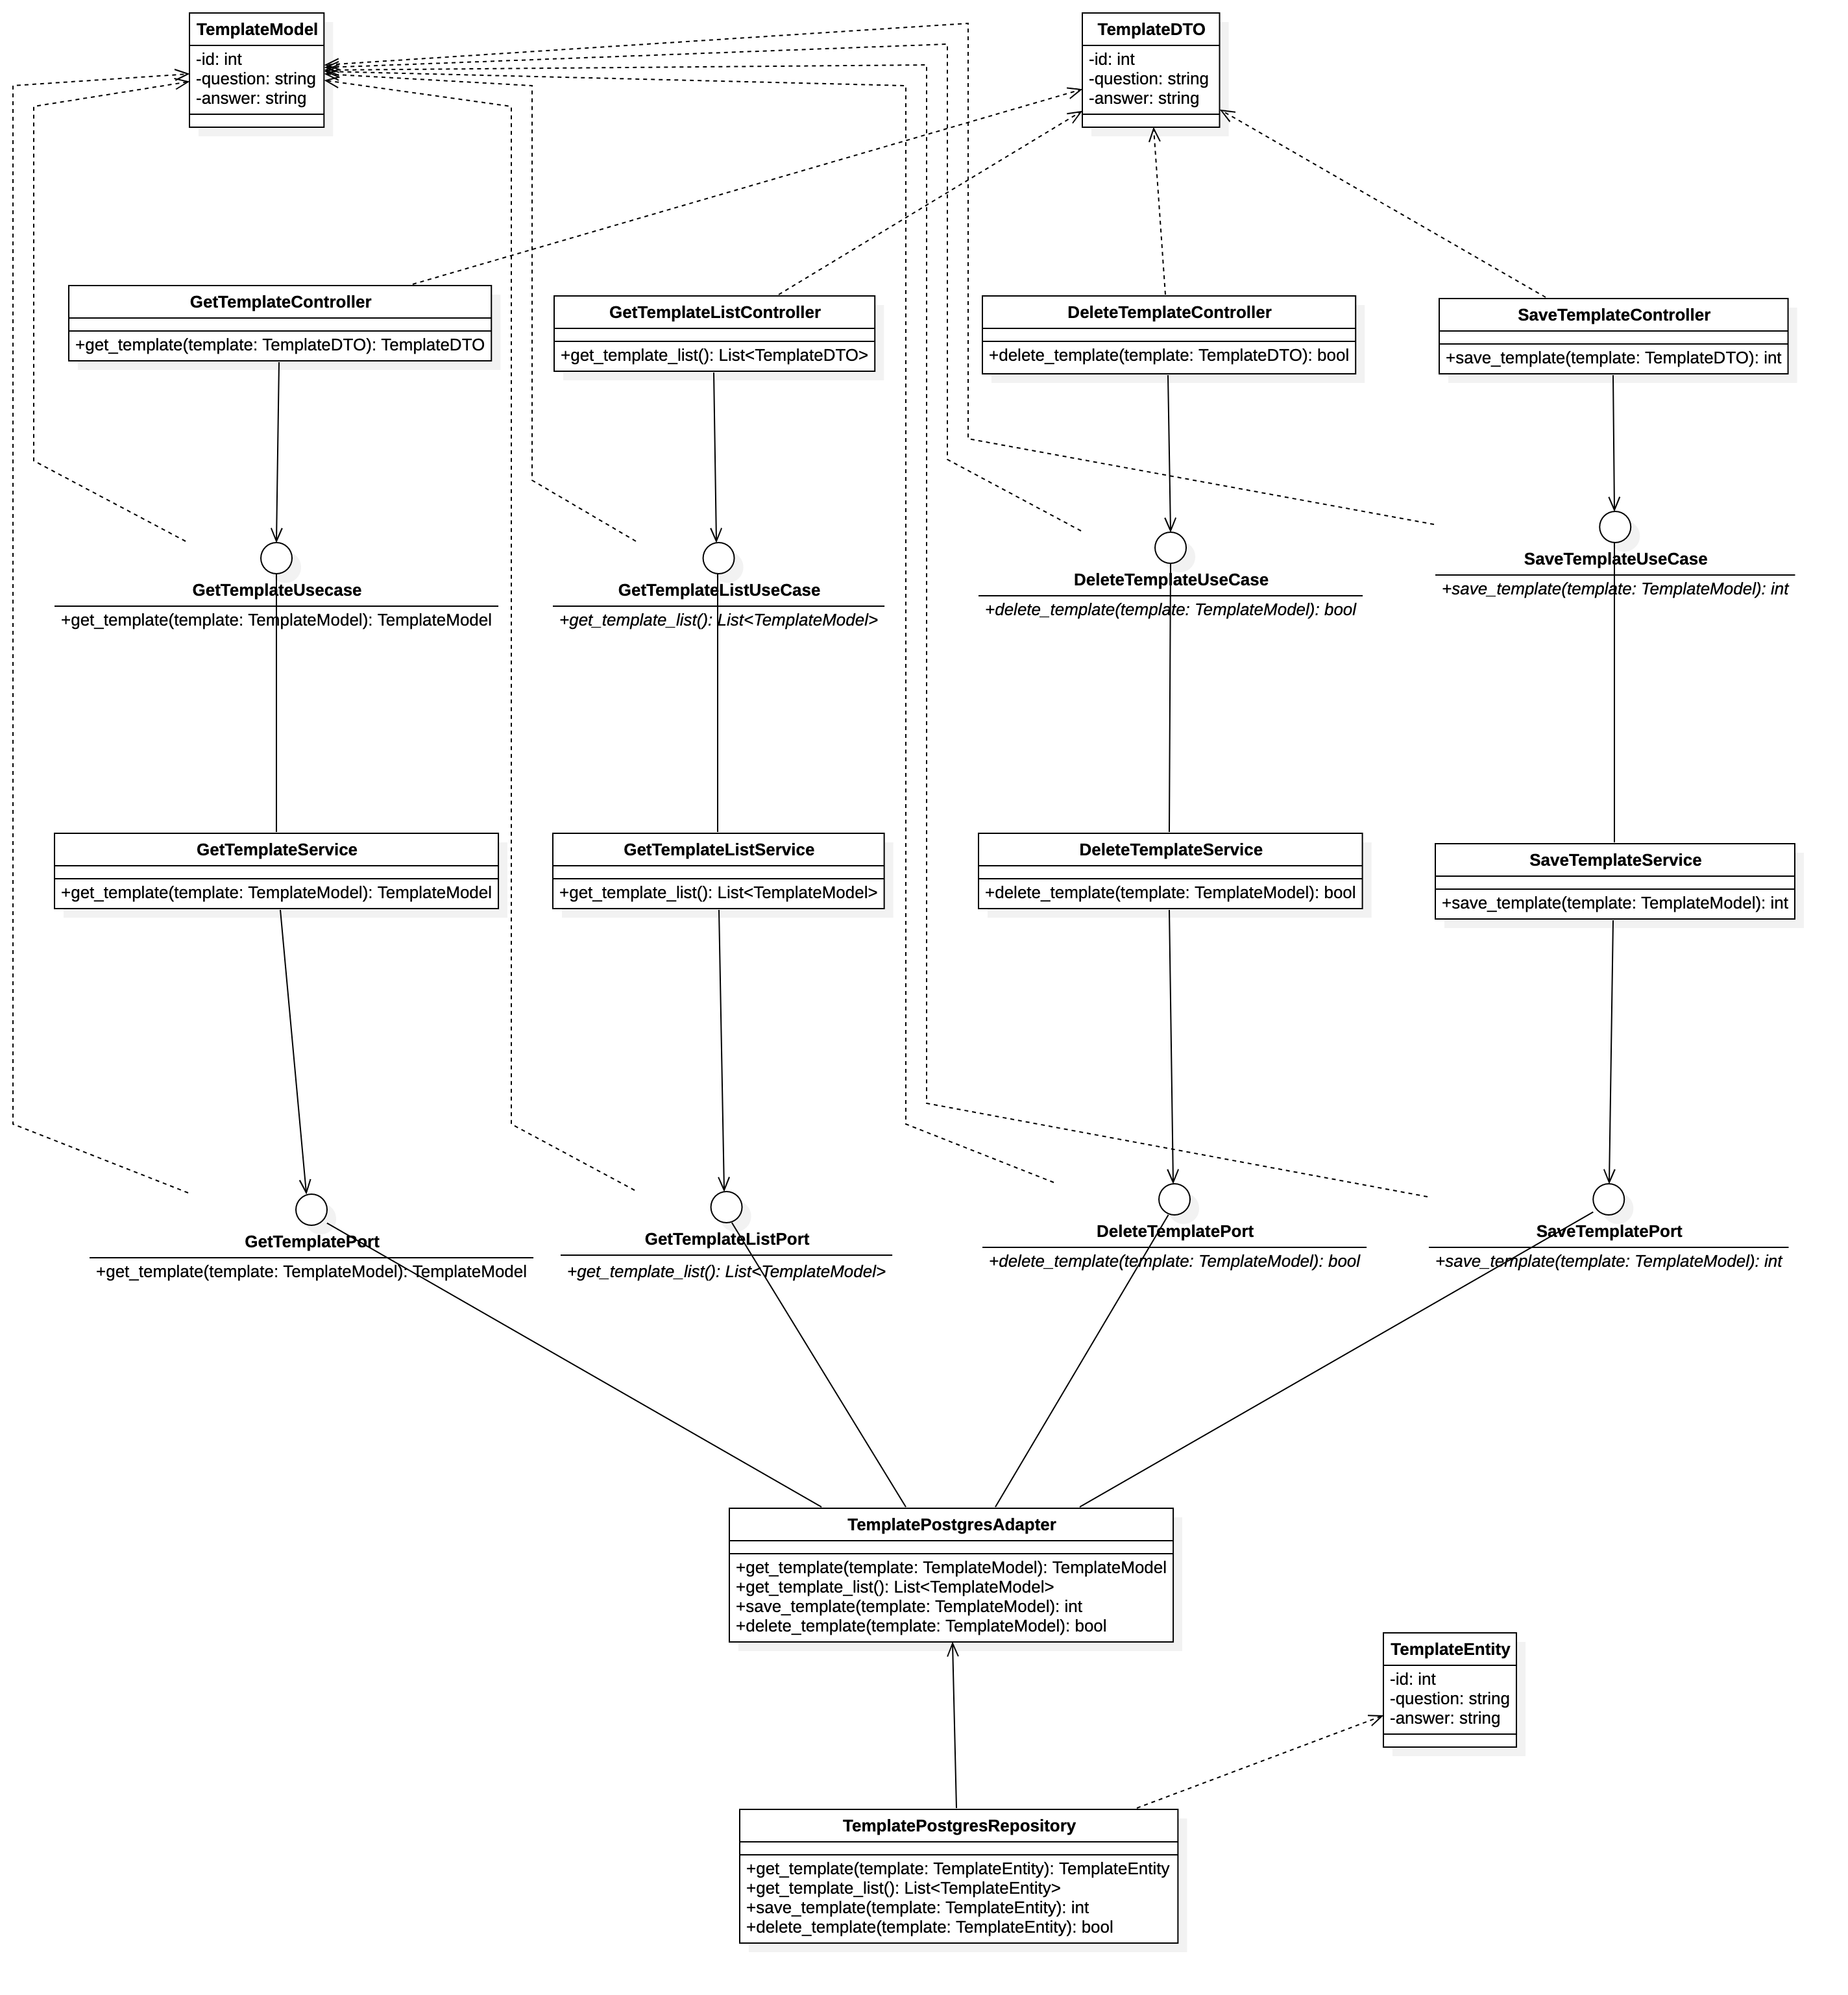
\includegraphics[width=\linewidth, height=0.8\textheight, keepaspectratio]{./img/Template.png}
        \caption{Diagramma delle classi - Template}
        \label{fig:template}
    \end{figure}

    Il modulo implementa un'architettura a più livelli per la gestione di "template" (che potrebbero rappresentare, ad esempio, dei modelli di domande/risposte) utilizzando i principi della separazione delle responsabilità, dell'iniezione delle dipendenze e dell'astrazione tramite interfacce. Di seguito viene descritto in dettaglio il funzionamento dei vari componenti:
    
    \paragraph{1. DTO, Model ed Entity}
    \begin{itemize}
        \item \textbf{TemplateDTO:}
        \begin{itemize}
            \item \textbf{Scopo:} È un Data Transfer Object, usato per trasferire dati tra i livelli dell’applicazione (ad esempio, dal controller al livello dei use case e viceversa).
            \item \textbf{Attributi:} id, question, answer, author\_id, last\_modified.
            \item \textbf{Metodi:} I metodi getter (ad esempio, get\_id(), get\_question(), ecc.) permettono di accedere ai dati incapsulati.
        \end{itemize}
        \item \textbf{TemplateModel:}
        \begin{itemize}
            \item \textbf{Scopo:} Rappresenta il modello di dominio all’interno del business logic. È simile al DTO ma viene usato internamente al sistema per manipolare i dati.
            \item \textbf{Attributi e metodi:} Gli stessi del DTO, facilitando la conversione e il passaggio dei dati tra i vari layer.
        \end{itemize}
        \item \textbf{TemplateEntity:}
        \begin{itemize}
            \item \textbf{Scopo:} Rappresenta l’oggetto persistente, ovvero il mapping della tabella del database (in questo caso, la tabella “Templates”).
            \item \textbf{Attributi e metodi:} Identici a quelli del DTO e del Model, ma utilizzati specificamente per interagire con il database.
        \end{itemize}
    \end{itemize}
    
    \paragraph{2. Controllers}
    I controller fungono da interfaccia tra le richieste dell’utente e i casi d’uso (use cases). Essi ricevono i dati sotto forma di DTO, li convertono in modelli, invocano il caso d’uso corrispondente e poi ritrasformano il risultato in DTO per la risposta.
    
    \begin{itemize}
        \item \textbf{GetTemplateController:}
        \begin{itemize}
            \item \textbf{Funzione:} Riceve un TemplateDTO e crea un TemplateModel corrispondente.
            \item \textbf{Processo:} Chiama il metodo get\_template del use case, controlla se il risultato è None e, in caso contrario, converte il TemplateModel ottenuto in un nuovo TemplateDTO da restituire.
        \end{itemize}
        \item \textbf{GetTemplateListController:}
        \begin{itemize}
            \item \textbf{Funzione:} Recupera l’elenco di tutti i template.
            \item \textbf{Processo:} Chiama il use case per ottenere la lista di TemplateModel e li trasforma in una lista di TemplateDTO mediante una list comprehension.
        \end{itemize}
        \item \textbf{SaveTemplateController:}
        \begin{itemize}
            \item \textbf{Funzione:} Salva un nuovo template.
            \item \textbf{Processo:} Converte il TemplateDTO in TemplateModel e invoca il use case per salvare il template. Il metodo restituisce l’ID del template salvato.
        \end{itemize}
        \item \textbf{DeleteTemplateController:}
        \begin{itemize}
            \item \textbf{Funzione:} Gestisce la cancellazione di un template.
            \item \textbf{Processo:} Converte il TemplateDTO in TemplateModel e chiama il metodo di cancellazione del use case, restituendo un booleano che indica il successo dell’operazione.
        \end{itemize}
    \end{itemize}
    
    \paragraph{3. Use Cases (Casi d’Uso) e Servizi}
    I use case definiscono le operazioni fondamentali (ad esempio, ottenere, salvare o cancellare un template) e sono dichiarati come classi astratte per garantire che le implementazioni concrete rispettino la firma definita.
    
    \begin{itemize}
        \item \textbf{Use Case Astratti:}
        \begin{itemize}
            \item \textbf{GetTemplateUseCase, GetTemplateListUseCase, SaveTemplateUseCase, DeleteTemplateUseCase:} Definiscono i metodi astratti che devono essere implementati. Essi forniscono la “contrattualità” per le operazioni che il sistema deve eseguire.
        \end{itemize}
    \end{itemize}
    
    \paragraph{4. Ports (Interfacce di Ingresso/Uscita)}
    I “ports” sono interfacce astratte che definiscono come il sistema comunica con l’esterno (ad esempio, il database). Permettono di disaccoppiare la logica di business dall’implementazione concreta della persistenza.
    
    \begin{itemize}
        \item \textbf{GetTemplatePort:} Definisce il metodo get\_template per ottenere un template.
        \item \textbf{GetTemplateListPort:} Definisce il metodo get\_template\_list per recuperare tutti i template.
        \item \textbf{SaveTemplatePort:} Definisce il metodo save\_template per salvare un template.
        \item \textbf{DeleteTemplatePort:} Definisce il metodo delete\_template per cancellare un template.
    \end{itemize}
    
    \paragraph{5. Adapter e Repository}
    \begin{itemize}
        \item \textbf{TemplatePostgresAdapter:}
        \begin{itemize}
            \item \textbf{Ruolo:} È un adattatore che implementa tutte le interfacce dei ports (Get, List, Save, Delete).
            \item \textbf{Funzionamento:}
            \begin{itemize}
                \item Converte un TemplateModel in un TemplateEntity (il formato richiesto dal repository) e viceversa.
                \item Invoca i metodi del TemplatePostgresRepository per eseguire le operazioni concrete sul database.
                \item Gestisce le conversioni per assicurare che il livello di business lavori con TemplateModel mentre il livello di persistenza lavora con TemplateEntity.
            \end{itemize}
        \end{itemize}
        \item \textbf{TemplatePostgresRepository:}
        \begin{itemize}
            \item \textbf{Scopo:} Fornisce l’accesso diretto al database PostgreSQL utilizzando il modulo psycopg2.
            \item \textbf{Metodi principali:}
            \begin{itemize}
                \item \_\_connect(): Stabilisce la connessione al database usando la configurazione fornita.
                \item get\_template(): Esegue una query per recuperare un template in base al suo ID. Se il template non viene trovato, viene sollevata un’eccezione.
                \item get\_template\_list(): Esegue una query per recuperare tutti i template dalla tabella "Templates" e li restituisce come lista di TemplateEntity.
                \item save\_template(): Esegue una query di INSERT per salvare un nuovo template. Dopo l’inserimento, restituisce l’ID generato.
                \item delete\_template(): Esegue una query di DELETE e controlla se almeno una riga è stata eliminata per determinare il successo dell’operazione.
            \end{itemize}
            L’utilizzo dei blocchi with assicura la corretta gestione della connessione e del cursore, mentre il commit della transazione viene eseguito solo se l’operazione di modifica ha avuto successo.
        \end{itemize}
    \end{itemize}
    
    \paragraph{Riassunto del Flusso dei Dati}
    \begin{enumerate}
        \item \textbf{Ricezione della richiesta:} Un client (ad esempio, un’API REST) invoca uno dei controller, passando un TemplateDTO (per operazioni individuali) o richiedendo una lista di template.
        \item \textbf{Conversione e invocazione del Use Case:} Il controller converte il DTO in un TemplateModel e chiama il relativo use case (implementato nei servizi).
        \item \textbf{Interazione con il livello di persistenza:} Il servizio, tramite il port, utilizza l’adapter (TemplatePostgresAdapter) per convertire il TemplateModel in TemplateEntity e invoca il metodo corrispondente del repository.
        \item \textbf{Esecuzione della query sul database:} Il repository stabilisce la connessione, esegue la query SQL, e restituisce il risultato (convertito in TemplateEntity).
        \item \textbf{Ritorno del risultato:} L’adapter converte l’entity in TemplateModel, il servizio lo passa al controller, che a sua volta lo trasforma in TemplateDTO per inviarlo come risposta al client.
    \end{enumerate}
    
    
    \subsubsection{Database}
    \begin{figure}[H]
        \centering
        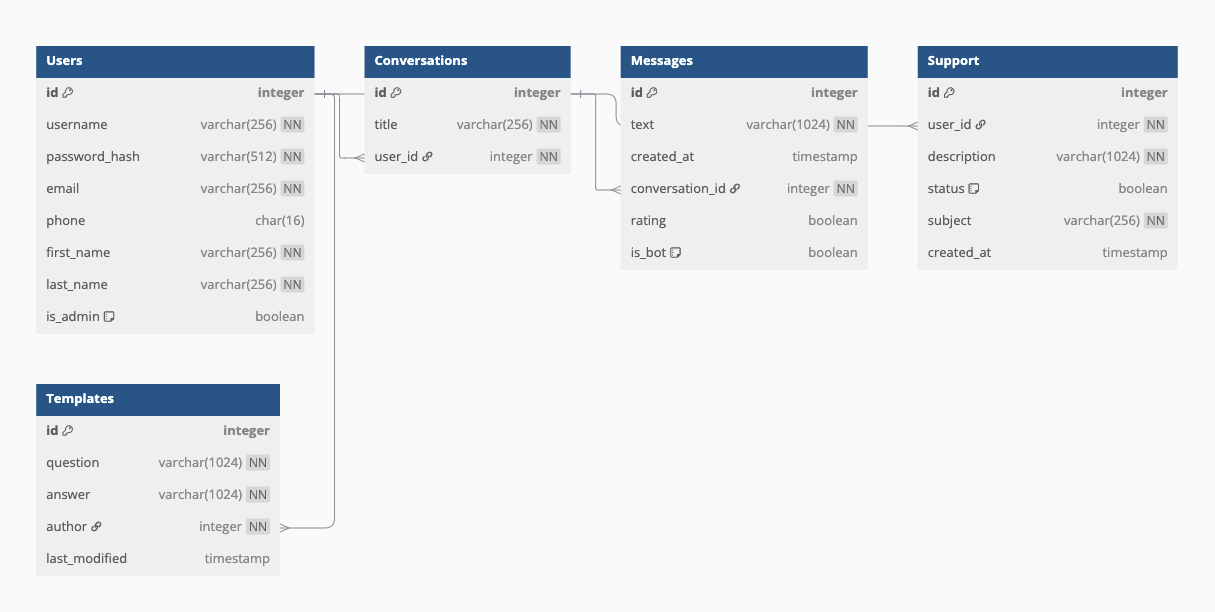
\includegraphics[width=\linewidth, height=0.8\textheight, keepaspectratio]{./img/DB_ER.png}
        \caption{Diagramma ER del Database}
        \label{fig:db_er}
    \end{figure}

    Il database è stato progettato per gestire una piattaforma che offre funzionalità di gestione utenti, conversazioni, messaggi, supporto e template. 
    L'obiettivo principale del database è garantire un'archiviazione efficiente e sicura dei dati relativi agli utenti e alle loro interazioni, oltre a supportare funzionalità di supporto tecnico e gestione di risposte preimpostate.
    La piattaforma è pensata per essere utilizzata da utenti comuni e amministratori, con la possibilità di distinguere tra messaggi generati manualmente e automaticamente (da bot). 
    Ogni conversazione può contenere uno o più messaggi, i quali possono essere valutati tramite un sistema di rating. 
    Inoltre, il database prevede una gestione centralizzata delle richieste di supporto e la possibilità di utilizzare template predefiniti per automatizzare risposte comuni.
    La struttura del database è stata pensata per garantire integrità e consistenza dei dati attraverso l'uso di vincoli di chiave esterna e l'eliminazione a cascata, in modo da mantenere la pulizia del database ed evitare riferimenti orfani. 
    Di seguito sono descritte nel dettaglio le principali tabelle e la loro struttura.


    \paragraph{Tabella Users} \mbox{} \\
    Questa tabella contiene le informazioni sugli utenti della piattaforma. I campi principali sono:
    \begin{itemize}
        \item \textbf{id}: Identificatore univoco dell'utente (generato automaticamente).
        \item \textbf{username}: Nome utente (unico).
        \item \textbf{password\_hash}: Hash della password (per la sicurezza).
        \item \textbf{email}: Indirizzo email (unico).
        \item \textbf{phone}: Numero di telefono (opzionale).
        \item \textbf{first\_name} e \textbf{last\_name}: Nome e cognome dell'utente.
        \item \textbf{is\_admin}: Flag per indicare se l'utente ha privilegi di amministrazione (valore predefinito: FALSE).
    \end{itemize}
    
    \paragraph{Tabella Conversations} \mbox{} \\
    Memorizza le conversazioni create dagli utenti. I campi principali sono:
    \begin{itemize}
        \item \textbf{id}: Identificatore univoco della conversazione.
        \item \textbf{title}: Titolo della conversazione.
        \item \textbf{user\_id}: Riferimento all’utente che ha creato la conversazione.
        \item Relazione con la tabella \textbf{Users}, con eliminazione a cascata.
    \end{itemize}
    
    \paragraph{Tabella Messages} \mbox{} \\
    Contiene i messaggi all’interno delle conversazioni. I campi principali sono:
    \begin{itemize}
        \item \textbf{id}: Identificatore univoco del messaggio.
        \item \textbf{text}: Contenuto del messaggio.
        \item \textbf{created\_at}: Data e ora di creazione (timestamp con fuso orario).
        \item \textbf{conversation\_id}: Riferimento alla conversazione a cui appartiene.
        \item \textbf{rating}: Valutazione del messaggio (booleano).
        \item \textbf{is\_bot}: Flag per indicare se il messaggio è generato da un bot (valore predefinito: FALSE).
        \item Relazione con la tabella \textbf{Conversations}, con eliminazione a cascata.
    \end{itemize}
    
    \paragraph{Tabella Support} \mbox{} \\
    Gestisce le richieste di supporto inviate dagli utenti. I campi principali sono:
    \begin{itemize}
        \item \textbf{id}: Identificatore univoco della richiesta.
        \item \textbf{user\_id}: Riferimento all’utente che ha inviato la richiesta.
        \item \textbf{description}: Descrizione del problema o della richiesta.
        \item \textbf{status}: Stato della richiesta (risolta o meno).
        \item \textbf{subject}: Oggetto della richiesta.
        \item \textbf{created\_at}: Data e ora della creazione della richiesta.
        \item Relazione con la tabella \textbf{Users}, con eliminazione a cascata.
    \end{itemize}
    
    \paragraph{Tabella Templates} \mbox{} \\
    Memorizza i template di domande e risposte create dagli utenti (ad esempio, bot o risposte preimpostate). I campi principali sono:
    \begin{itemize}
        \item \textbf{id}: Identificatore univoco del template.
        \item \textbf{question} e \textbf{answer}: Testo della domanda e della risposta associata.
        \item \textbf{author}: Riferimento all’utente che ha creato il template.
        \item \textbf{last\_modified}: Timestamp dell’ultima modifica.
        \item Relazione con la tabella \textbf{Users}, con eliminazione a cascata.
    \end{itemize}
    
    \paragraph{Eliminazione delle Tabelle} \mbox{} \\
    Sono presenti anche delle query per eliminare tutte le tabelle e i relativi dati in modo sicuro e completo usando il comando \texttt{DROP TABLE IF EXISTS ... CASCADE}.
    





\subsection{Tecnologie}
%%%%%%%%%%%%%%%%%%%%%%%%%%%%%%%%%%%%%%%%%%%%%%%%%%%%%%%%%%%%%%%%%%%%%%%%%%%%%%%%%%
\subsubsection{OpenAI API}
%%%%%%%%%%%%%%%%%%%%%%%%%%%%%%%%%%%%%%%%%%%%%%%%%%%%%%%%%%%%%%%%%%%%%%%%%%%%%%%%%%

